% =============================================================================
%  T-RO extension of "Geometry-Aware Control Barrier Functions for Collision
%  Avoidance via Bernstein Polynomial Approximations" (ICRA 2026, arXiv:2605.30696)
%
%  Numbers come from the scripts in the parent folder:
%     cspace_sdf_cbf_compare.py, cspace_cbf_5robots.py, cspace_experiments.py  (planar, compiled field)
%     prototype_3d/dock_cover.py, prototype_3d/five_cover.py, maze_cover.py     (planar, surface cover)
%     prototype_3d/summed.py, summed3d.py: summed-field barriers with Bernstein coefficient constraints
%       (Sec. IV; checks: summed_check.py, summed_check2d.py). The previous corner barriers (safe set
%       depending on the boxes) remain available with --corner / method 'corner'; their results are in
%       *_corner.json, results/reference_maze_cover/, and tro/figs_corner_backup/.
%     make_paper_figs.py overview|dock2|five, reference_maze_escape.py         (Figs. 1-4)
%     prototype_3d/franka3d.py, prototype_3d/franka_fig.py                     (Franka, Sec. VIII-G)
%  Raw results: ../results/*.json, ../prototype_3d/franka_results.json
%  Planar timings: one CPU thread (OMP/MKL/OPENBLAS_NUM_THREADS=1), nothing else running.
%  The previous planar-only manuscript is kept as main_planar_long_2026-09-27.tex; the version with the
%  tabulated field as the main planar construction as main_before_cover_first_2026-09-28.tex.
%
%  Double-anonymous review: \anonymoustrue hides the authors and the running head; the prior
%  conference paper and the ICRA'27 manuscript are cited in the third person and supplied to the
%  editor. Set \anonymousfalse for the final version.
%
%  OPEN ITEMS (kept out of the PDF):
%   - Franka: franka3d.py 30, franka_baselines.py spheres points kkt [--margin 0], dual3d.py 20
%     (prototype_3d/franka_results.json, franka_baselines.json, dual_results.json)
%   - planar docking with the surface cover: cspace_experiments.py dock2 (all barriers), dock_cover.py 5 2.5
%   - five robots with the surface cover: prototype_3d/five_cover.py stats 5, swap 5
%   - confirm author list/order and affiliations with all co-authors
%   - cover letter: relation to [jo2026geometry] (authors' own) and to [jo2027semantic] (under review)
%   - planar comparison of the two constructions; manipulator baselines; hardware
% =============================================================================
\documentclass[journal]{IEEEtran}

\usepackage{amsmath,amssymb,amsthm}
\usepackage{graphicx}
\usepackage{booktabs}
\usepackage{algorithm}
\usepackage{algpseudocode}
\usepackage{xcolor}
\usepackage{cite}

\newtheorem{theorem}{Theorem}
\newtheorem{lemma}{Lemma}
\newtheorem{proposition}{Proposition}
\newtheorem{corollary}{Corollary}
\newtheorem{assumption}{Assumption}
\theoremstyle{definition}
\newtheorem{definition}{Definition}
\newtheorem{remark}{Remark}

\newcommand{\R}{\mathbb{R}}
% step times measured in isolation by prototype_3d/franka_timing.py (median / 95th percentile, ms)
\newcommand{\timeFrankaMed}{13.3}\newcommand{\timeFrankaPninetyfive}{46.5}
\newcommand{\timeDualMed}{7.6}\newcommand{\timeDualPninetyfive}{78}
\newcommand{\timeOurs}{13.3/46.5}\newcommand{\timeSph}{1.9/3.7}\newcommand{\timePts}{3.3/7.1}\newcommand{\timeKKT}{128/487}
\newcommand{\Sone}{\mathbb{S}^1}
\newcommand{\norm}[1]{\left\lVert #1\right\rVert}
\newcommand{\CO}{\mathcal{C}}
\newcommand{\Mset}{\mathcal{M}}
\newcommand{\Rot}{\mathbf{R}}
\DeclareMathOperator{\conv}{conv}
\DeclareMathOperator*{\argmin}{arg\,min}

\graphicspath{{figs/}}

\newif\ifanonymous
\anonymoustrue

\begin{document}

\title{Certified Geometry-Aware Control Barrier Functions for Non-Convex Rigid and Articulated
Robots}

\ifanonymous
\author{Anonymous Authors}
\markboth{IEEE Transactions on Robotics}%
{Certified Geometry-Aware Control Barrier Functions for Non-Convex Robots}
\else
\author{Siwon~Jo, Yanze~Zhang, Yupeng~Yang, and~Wenhao~Luo%
\thanks{A preliminary version of this work appeared at the IEEE International Conference on
Robotics and Automation (ICRA), 2026~\cite{jo2026geometry}. Section~\ref{sec:relation}
summarizes the differences.}%
\thanks{S.~Jo is with the GRASP Laboratory, University of Pennsylvania, Philadelphia, PA 19104,
USA. Y.~Zhang and W.~Luo are with the Department of Computer Science, University of Illinois
Chicago, Chicago, IL 60607, USA. Y.~Yang is with the Department of Computer Science, University
of North Carolina at Charlotte, Charlotte, NC 28223, USA.}}

\markboth{IEEE Transactions on Robotics}%
{Jo \MakeLowercase{\textit{et al.}}: Certified Geometry-Aware Control Barrier Functions for Non-Convex Robots}
\fi

\maketitle

% -----------------------------------------------------------------------------
\begin{abstract}
Geometry-aware control barrier functions (CBFs) that evaluate signed distance fields (SDFs) at
closest boundary points need convex level sets, treat non-convex geometry through rotation-invariant
bounding circles, and rely on a heuristic enclosure margin. We show that collision avoidance between
non-convex rigid bodies reduces to a condition on their boundaries at first contact. Each body's SDF
is a B-spline whose enclosing level is certified on the continuous boundary, and the safe set
requires the SDF of one body to stay above its level on the certified level set of the other. This
level set is covered offline by boxes selected from Bernstein coefficients; online, each box yields
finitely many constraints affine in the inputs, from Bernstein and vertex bounds of a lifted barrier,
without closest points. The safe set is not discretized: the boxes only restrict the admissible
inputs, by an amount of second order in the box size. The construction applies to planar and
spatial, rigid and articulated bodies; planar pairs can instead be compiled into one certified
configuration-space field. In simulation, both constructions prevented all collisions of non-convex
rotating robots, unlike a closest-point barrier, and docked where bounding circles cannot. A Franka
Panda avoided three non-convex obstacles in all 30 trials in which the unfiltered motion collides,
coming within 1.1~mm, whereas a closest-point barrier collided in 7 and margin-free sphere and
surface-sample barriers in 17 and 19; two Pandas kept their meshes apart. The price of the exact
safe set is slower motion near contact and a higher cost per step.
\end{abstract}

\begin{IEEEkeywords}
Collision avoidance, control barrier functions, signed distance fields, configuration space,
Bernstein polynomials, B-splines, multi-robot systems, manipulators.
\end{IEEEkeywords}

% -----------------------------------------------------------------------------
\section{Introduction}\label{sec:intro}

\IEEEPARstart{C}{ontrol} barrier functions (CBFs)~\cite{ames2019cbf} turn safety conditions into
constraints on the control input, typically enforced by a quadratic program (QP) that minimally
modifies a nominal command. For collision avoidance, their value is determined by the geometric
surrogate behind the barrier. Spheres and super-ellipsoids~\cite{wang2017safety,wang2017quadrotors}
are smooth but conservative for irregular shapes; polytopic
formulations~\cite{chen2025minkowski,thirugnanam2025strongly} are exact for convex pieces but become
pairwise and piecewise for non-convex bodies; learned, point-cloud, and sampled
barriers~\cite{khan2022gaussian,long2021learning,dai2024sailing,lutkus2025sampling} trade exactness
for generality.

Jo et al.~\cite{jo2026geometry} proposed geometry-aware CBFs on Bernstein-polynomial
SDFs~\cite{li2024representing}: the barrier is the robot's SDF evaluated at the closest point of the
obstacle boundary, obtained from the Karush--Kuhn--Tucker (KKT) conditions. That formulation has
three limitations. \emph{L1)} Its time derivative requires the closest point to move smoothly, which
holds only for convex level sets. \emph{L2)} For composite or non-convex geometry, the closest point
jumps and the barrier is non-smooth; the remedy of~\cite{jo2026geometry}, inflating obstacles by
the robot's bounding circle, ignores orientation. \emph{L3)} The enclosure of the true geometry by
the fitted level set rests on a user-chosen margin.

This article removes all three. Its starting point is that two compact bodies can only begin to
intersect at a point that lies on both boundaries (Lemma~\ref{lem:contact}). Keeping the SDF of one
body above its level on the whole boundary of the other therefore suffices, and no closest point is
needed. This condition on the continuous certified boundary is our safe set, which we
\emph{enforce} online: the boundary of one body is covered by small boxes, and on each box a lifted
barrier, which adds the body's own SDF, yields finitely many constraints affine in the inputs that
suffice at every point of the box (Fig.~\ref{fig:overview}b). The boxes enter only the constraints on
the inputs, never the safe set, and their effect is of second order in the box size. The construction
needs one field per body, not per pair,
and applies unchanged to planar and spatial bodies and to articulated robots. For planar pairs, whose
relative pose is only three-dimensional, the minimum can instead be \emph{compiled} offline into one
smooth field over $(x,y,\theta)$ per pair (Fig.~\ref{fig:overview}c); a single scalar barrier then
encodes non-convex shapes and rotation, at the price of a level that absorbs the error of the
training data.

\begin{figure*}[t]
\centering
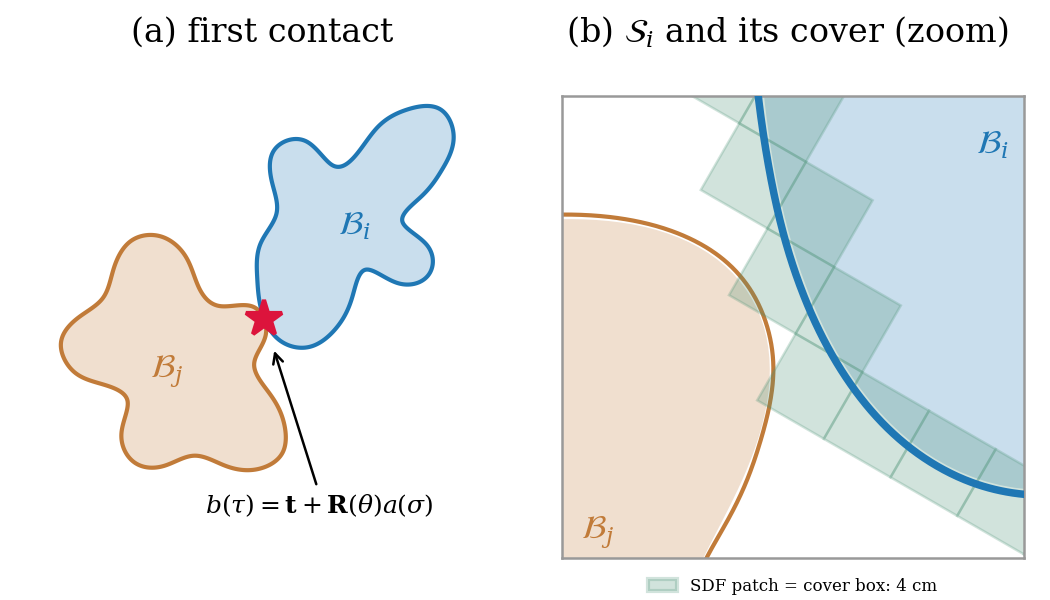
\includegraphics[width=\textwidth]{overview.png}
\caption{Both constructions for two planar bodies. (a) Every first contact occurs at a
configuration $\mathbf t=b(\tau)-\Rot(\theta)a(\sigma)$ that joins boundary points of both bodies
(Lemma~\ref{lem:contact}). (b) Surface cover (Sec.~\ref{sec:cover}), with $\mathcal B_i$ 3~cm before
contact: the safe set requires $\mathcal B_j$'s SDF to stay above its certified level set (orange) on
every point of the continuous certified curve $\mathcal S_i$ (thick blue); the 5-mm boxes that cover
$\mathcal S_i$ (faint; filled: boxes carrying constraints) only partition it to generate the
constraints on the inputs; fills: ground truth. (c) Compiled field (Sec.~\ref{sec:tab}): the configuration-space obstacle
$\CO_{ij}$ (gray: rasterized reference, eight orientations) and the certified level set
$\{\phi_{ij}=l^\star_{ij}\}$ of one B-spline field over $SE(2)$ (orange).}
\label{fig:overview}
\end{figure*}

\subsection{Contributions}
\begin{enumerate}
\item \emph{Boundary reduction and certified regions} (Sec.~\ref{sec:regions}): a first-contact
lemma for compact bodies in $\R^n$, and certified levels of fitted SDFs that enclose the true
geometry, for spline boundaries and for triangle meshes (resolves L3).
\item \emph{Surface-cover barriers} (Sec.~\ref{sec:cover}): a safe set defined on the continuous level
set of each body's SDF, enforced through Bernstein and vertex constraints on a lifted barrier over a
Bernstein cover of that level set, with certified Taylor remainders from third-derivative bounds;
the constraints are affine in the inputs of planar robots and in the joint velocities of
manipulators, their conservatism is of second order in the box size and falls on the inputs only, and
no closest points or online optimization are needed (resolves L1 and L2).
\item \emph{Compiled barrier for planar pairs} (Sec.~\ref{sec:tab}): one smooth barrier per pair of
non-convex rotating bodies over $SE(2)$, whose level is certified on the explicit three-parameter
first-contact set by a Bernstein branch-and-bound, together with certificates of its activation
band and regularity.
\item \emph{Evaluation} (Sec.~\ref{sec:exp}): planar docking, multi-robot, and static-obstacle
experiments with both constructions under single-integrator and unicycle dynamics against
closest-point, bounding-circle, sampling-based, and ball-world baselines, a comparison of
Bernstein-form representations, a 7-DOF Franka Panda among non-convex obstacles against sphere and
surface-sample barriers, and two Pandas in a shared workspace.
\end{enumerate}

\subsection{Relation to Prior Work}\label{sec:relation}
This article keeps the problem formulation, the Bernstein-form distance fields, the pairwise
multi-robot QP, and the experimental protocol of~\cite{jo2026geometry}. It replaces the
closest-point barrier (retained as a baseline), the bounding-circle configuration space, and the
heuristic margin. New are the first-contact reduction, both barrier constructions with their
certificates and derivatives, the feasibility result, the representation analysis, and all
experiments. The certified enclosure of planar boundaries by B-spline curves and the conversion of
B-splines to Bernstein form follow~\cite{jo2027semantic} and are not claimed as contributions.

% -----------------------------------------------------------------------------
\section{Related Work}\label{sec:related}

\emph{Geometric barriers.} Pairwise barriers between discs or spheres are the standard multi-robot
certificates~\cite{wang2017safety}, and super-ellipsoids extend them to elongated
vehicles~\cite{wang2017quadrotors}; unions of primitives multiply the constraints. For convex
polytopes, signed distances through convex programs in the Minkowski-difference space yield exact
barriers~\cite{chen2025minkowski,chen2026exact}, and smooth barriers exist between strongly convex
regions~\cite{thirugnanam2025strongly}; non-convex bodies must be decomposed. Explicit smooth
barriers for polygons compose edge-wise bounds with smooth extrema~\cite{wu2025optimization}.
Sampled distance functions yield nonsmooth barriers with quantified sampling
error~\cite{lutkus2025sampling}, and diffeomorphisms to ball worlds handle non-convex unsafe sets
without undesired equilibria~\cite{notomista2021nonconvex}; we compare with adaptations of both.

\emph{Distance fields for manipulators.} Bernstein-polynomial distance fields of articulated robots
support whole-body collision avoidance, with obstacle points queried against the robot
field~\cite{li2024representing}; neural configuration-space distance functions serve as CBFs with
robust margins~\cite{long2025neural}, and differentiable distance fields map obstacle motion into
joint space~\cite{chi2024safe}. These works establish distance fields as barriers; they do not
certify that the constraint holds on the whole continuous surface of the fitted or true geometry,
which is what our surface covers provide.

\emph{Configuration-space obstacles and Bernstein bounds.} Configuration-space obstacles of polygons
can be constructed exactly~\cite{lozanoperez1983spatial,latombe1991robot} or by grid
convolution~\cite{kavraki1995fft}; we use the latter only to produce training data. The
convex-hull property and de~Casteljau subdivision give rigorous, successively tighter bounds on
polynomials over boxes~\cite{farin2002curves,sherbrooke1993computation}; they were used
in~\cite{jo2027semantic} to certify planar spline enclosures, and we use them in up to three
variables on tensor-product fields.

% -----------------------------------------------------------------------------
\section{Preliminaries and Problem Statement}\label{sec:prelim}

\emph{CBFs.} Consider $\dot{\mathbf z}=f(\mathbf z)+g(\mathbf z)\mathbf u$ with $f,g$ locally
Lipschitz, $\mathbf u\in\mathcal U$, and a $C^1$ function $h$ with
$\mathcal H=\{\mathbf z\mid h(\mathbf z)\ge0\}$.
\begin{lemma}[\cite{ames2019cbf}]\label{lem:cbf}
If a locally Lipschitz feedback $\mathbf k(\mathbf z)\in\mathcal U$ satisfies
$L_fh+L_gh\,\mathbf k\ge-\gamma h$ with $\gamma>0$ on an open set containing $\mathcal H$, then
$\mathcal H$ is forward invariant.
\end{lemma}

\emph{Bernstein form.} The cubic Bernstein basis $B_r(\xi)=\binom3r\xi^r(1-\xi)^{3-r}$ is
nonnegative and sums to one, so $p=\sum_r\beta_rB_r$ satisfies $\min_r\beta_r\le p\le\max_r\beta_r$
on $[0,1]$ (convex-hull property), also for tensor products. With $M_B$ mapping Bernstein to power
coefficients and $T_{jr}=\binom rj\xi_0^{r-j}\Delta^j$ ($j\le r$), the coefficients of $p$ restricted
to $[\xi_0,\xi_0+\Delta]$ and reparametrized to $[0,1]$ are
\begin{equation}\label{eq:subdiv}
\boldsymbol\beta'=S(\xi_0,\xi_0+\Delta)\,\boldsymbol\beta,\qquad S=M_B^{-1}T(\xi_0,\Delta)M_B,
\end{equation}
applied along each axis; they converge to the values of $p$ as $\Delta\to0$. On each span, a uniform
cubic B-spline with control values $\mathbf P_c,\dots,\mathbf P_{c+3}$ has Bernstein coefficients
\begin{equation}\label{eq:b2b}
\boldsymbol\beta_c=Q\,[\mathbf P_{c},\dots,\mathbf P_{c+3}]^{\top},\quad
Q=\tfrac16\left[\begin{smallmatrix}1&4&1&0\\0&4&2&0\\0&2&4&0\\0&1&4&1\end{smallmatrix}\right],
\end{equation}
so bounds on a tensor-product spline, and on its derivatives, follow from finitely many
coefficients per cell~\cite{farin2002curves,jo2027semantic}.

\emph{Problem.} Robot bodies and obstacles are compact sets $\mathcal G_i\subset\R^n$, $n\in\{2,3\}$
(the \emph{ground truth}, not necessarily convex), rigidly attached to frames with poses
$(\Rot_i,\mathbf p_i)$ that depend on the state: the pose of a mobile robot, or the forward
kinematics of a link. Given nominal inputs, find minimally modified inputs under which no two
bodies ever intersect, with constraints whose correctness is certified rather than sampled.

% -----------------------------------------------------------------------------
\section{Certified Regions and First Contact}\label{sec:regions}

\subsection{First Contact}
\begin{lemma}[First contact]\label{lem:contact}
Let $\mathcal K_A(s),\mathcal K_B(s)\subset\R^n$, $s\in[0,T]$, be images of compact sets under rigid
motions that are continuous in $s$, disjoint at $s=0$ and intersecting at $s=T$. Then at
$s^\star=\inf\{s\mid\mathcal K_A(s)\cap\mathcal K_B(s)\neq\emptyset\}>0$, some point lies on both
boundaries, $\partial\mathcal K_A(s^\star)\cap\partial\mathcal K_B(s^\star)\neq\emptyset$.
\end{lemma}
\begin{proof}
The set of intersecting parameters is closed, so the bodies intersect at $s^\star>0$; pick $\mathbf z$
in both. If $\mathbf z$ were interior to $\mathcal K_B(s^\star)$, the point of $\mathcal K_A$ that
is at $\mathbf z$ at $s^\star$ would, by continuity, lie in $\mathcal K_B(s)$ for $s<s^\star$ close
to $s^\star$, a contradiction. Symmetrically, $\mathbf z$ is not interior to $\mathcal K_A(s^\star)$,
since the point of $\mathcal K_B$ at $\mathbf z$ would lie in $\mathcal K_A$ before $s^\star$.
\end{proof}
The lemma requires neither convexity nor smoothness. It reduces collision avoidance to excluding
coincident boundary points, provided that the trajectory starts collision-free.

\subsection{Certified Regions}\label{sec:cert-body}
Each body is replaced by a region $\mathcal B_i\supseteq\mathcal G_i$ described by a fitted smooth
function whose enclosure of $\mathcal G_i$ is certified---a sublevel set of an SDF for the surface
cover, the inside of a spline curve for the compiled field---and safety for the regions then implies
safety for the ground truth.

\emph{Level sets of SDFs.} Let $\phi_i$ be a tensor-product cubic B-spline fitted to (approximate)
signed distances of $\mathcal G_i$ on a box $\Omega_i$, and let $\kappa_i(\mathbf c)$ be a certified
bound on $\norm{\nabla^2\phi_i}$ over the ball of radius $\rho\le h$ (the cell size) around $\mathbf c$: a
cubic B-spline whose control value $m$ is the maximum of the cellwise bounds from the Bernstein
coefficients of the second derivatives over cells $m-4,\dots,m+1$ per axis, which is $C^2$ and, its
weights being a partition of unity, bounds every cell adjacent to that of $\mathbf c$. The smallest level that encloses the boundary is
$\bar l_i=\max_{\partial\mathcal G_i}\phi_i$, and we certify it by branch-and-bound over pieces of the
boundary: triangles for a mesh, edges for a polygon, and, for a body given by an exact SDF, boxes of an
octree that may contain boundary points. For a piece $\mathcal T$ with center $\mathbf c$ and radius
$\rho$ (every point within $\rho$ of $\mathbf c$), Taylor's theorem gives
\begin{equation}\label{eq:level-ub}
\max_{\mathcal T}\phi_i\le\mathrm{UB}(\mathcal T)=\phi_i(\mathbf c)+\norm{\nabla\phi_i(\mathbf c)}\rho
+\tfrac12\kappa_i(\mathbf c)\rho^2 ,
\end{equation}
and $\phi_i$ at vertices, centers, or projected points on $\partial\mathcal G_i$ gives attained values
whose maximum $\ell$ lower-bounds $\bar l_i$. Pieces with $\mathrm{UB}<\ell+\epsilon$ are discarded;
the others are split (a triangle into four, an edge or a box into halves or octants) and re-bounded.
\begin{proposition}\label{prop:level}
When no piece is left, $l_i=\ell+\epsilon$ satisfies $\partial\mathcal G_i\subset\{\phi_i<l_i\}$ and
$l_i\le\bar l_i+\epsilon$. The procedure terminates for every $\epsilon>0$.
\end{proposition}
\begin{proof}
Every boundary point lies in a discarded piece, where $\phi_i\le\mathrm{UB}<\ell+\epsilon$ with $\ell$
nondecreasing, and $\ell\le\bar l_i$ because it is attained. Splitting halves $\rho$, and
$\mathrm{UB}-\phi_i(\mathbf c)\le G\rho+\tfrac12\kappa\rho^2\to0$ with $\phi_i(\mathbf c)\le\ell$ for
centers on the boundary (for octree boxes, $\phi_i(\mathbf c)\le\bar l_i+G\rho$), so every piece is
discarded after finitely many splits.
\end{proof}
The certificate is on the whole continuous boundary, is tight up to $\epsilon$, and needs no
sampling or distance computation; the fit affects only the size of $l_i$, never its validity, so the
training targets may be approximate. For the surface cover, $\mathcal B_i=\{\phi_i\le l_i\}$, and we
write $\mathcal S_i=\{\phi_i=l_i\}$ for the \emph{certified surface}.

\emph{Planar spline boundaries}~\cite{jo2027semantic}, used by the compiled field. The boundary is a closed periodic cubic
B-spline $a_i:\Sone\to\R^2$, fitted to outward-offset samples of $\mathcal G_i$ and accepted only if
every B\'ezier control hull (after subdivision) misses $\mathcal G_i$ and the curve winds around a
point of $\mathcal G_i$. The region $\mathcal B_i$ is the curve with the points of nonzero winding
number; for connected $\mathcal G_i$, $\mathcal G_i\subseteq\mathcal B_i$ and
$\partial\mathcal B_i\subseteq a_i(\Sone)$.

% -----------------------------------------------------------------------------
\section{Surface-Cover Barriers}\label{sec:cover}
We keep one SDF per body and enforce the first-contact condition on the whole certified surface; the
construction is the same for planar and spatial bodies, rigid or articulated. Let body $A$ (e.g., a
robot or a link) have the certified surface $\mathcal S_A=\{\phi_A=l_A\}$ in its frame, and let body $B$
(e.g., another robot or an obstacle) have the field $\phi_B$ and level $l_B$ in its frame, both from
Proposition~\ref{prop:level}. We write $\mathbf y(\mathbf x)$ for a point $\mathbf x$ of $A$ mapped into
$B$'s frame by the current relative pose. For planar bodies, the fields are bivariate and the boxes
below are squares.

\subsection{Safe Set on the Continuous Surface}
The safe set is the first-contact condition on every point of the certified surface,
\begin{equation}\label{eq:safe}
\mathcal H_{AB}=\big\{\text{poses}\ \big|\ h(\mathbf x)=\phi_B(\mathbf y(\mathbf x))-l_B\ge0\ \ \forall\mathbf x\in\mathcal S_A\big\};
\end{equation}
no box, sample, or bound enters its definition.
\begin{theorem}\label{thm:cover}
Suppose $\{\phi_A\le l_A\}$ and $\{\phi_B\le l_B\}$ are compact subsets of their domains, the bodies
start with $\{\phi_A\le l_A\}\cap\{\phi_B<l_B\}=\emptyset$, and a continuous trajectory stays in
$\mathcal H_{AB}$. Then $\mathcal G_A$ and $\mathcal G_B$ never intersect.
\end{theorem}
\begin{proof}
For $\epsilon>0$, if $\{\phi_A\le l_A\}$ met $\{\phi_B\le l_B-\epsilon\}$, Lemma~\ref{lem:contact} would
give a first point on both boundaries, where $\phi_A=l_A$ and $\phi_B=l_B-\epsilon$, contradicting
$h\ge0$ on $\mathcal S_A$. Hence $\{\phi_A\le l_A\}\cap\{\phi_B<l_B\}=\emptyset$ throughout. A first
contact of $\mathcal G_A$ and $\mathcal G_B$ would lie on $\partial\mathcal G_A\cap\partial\mathcal G_B$
(Lemma~\ref{lem:contact}), where $\phi_A<l_A$ and $\phi_B<l_B$ by Proposition~\ref{prop:level}.
\end{proof}

\subsection{Certified Cover and Lifted Barrier}
On each cell of $\phi_A$, the Bernstein coefficients of $\phi_A-l_A$ follow from~\eqref{eq:b2b}. If
they all have one strict sign on a box, the box contains no point of $\mathcal S_A$ by the
convex-hull property. Starting from the cells and halving every box whose coefficients change sign,
restricted by~\eqref{eq:subdiv}, until its side is at most $s_{\max}$, yields finitely many boxes
$\{\mathcal Q_k\}$ of side $s$, with centers $\mathbf c_k$ and half-diagonal $r$, whose union contains
all of $\mathcal S_A$, not a sample of it. The cover is computed once per body; it only partitions
the surface for the enforcement below and does not enter~\eqref{eq:safe}.

By the comparison lemma, $\mathcal H_{AB}$ stays invariant if $\dot h(\mathbf x)\ge-\gamma h(\mathbf x)$
at every surface point. The surface is implicit, so we impose this condition on whole boxes, after
lifting the barrier so that the points of a box off the surface do not tighten it: for $\mathbf x$ in a
box,
\begin{equation}\label{eq:lift}
\tilde h(\mathbf x)=\phi_A(\mathbf x)-l_A+\phi_B(\mathbf y(\mathbf x))-l_B ,
\end{equation}
which equals $h$ on $\mathcal S_A$. Since $\mathbf x$ is fixed in $A$'s frame, $\phi_A(\mathbf x)$ does
not change, and $\dot{\tilde h}(\mathbf x)=\nabla\phi_B(\mathbf y)^\top\dot{\mathbf y}(\mathbf x)$. A
box point displaced from the surface by $\delta$ toward $B$ has $\phi_A-l_A\approx\delta$ and
$\phi_B-l_B\approx h-\delta$ for SDF-like fields, so $\tilde h\approx h$: the lifting cancels the
first-order effect of the box size. The box points move with
$\dot{\mathbf y}(\mathbf x)=\mathbf J\mathbf u+\mathbf W(\mathbf u)(\mathbf y-\mathbf y_{\mathbf c})$,
affine in the inputs $\mathbf u$, where $\mathbf J\mathbf u$ is the velocity of the box center in
$B$'s frame and $\mathbf W(\mathbf u)$ the relative angular velocity as a skew matrix
(Sec.~\ref{sec:cover-der}).

\subsection{Bernstein and Vertex Constraints}
Cellwise bounds on the Frobenius norm of the third-derivative tensor follow from the Bernstein
coefficients of the third partial derivatives. A cubic B-spline is $C^2$ with piecewise-constant third
derivatives, so its Hessian is Lipschitz with these bounds on any region they cover, which is what the
third-order Taylor remainders below require. On each (fixed) box of $A$, $M_A$ is their maximum over
the at most $2^n$ cells meeting the box. For $\phi_B$, the bound must vary continuously with the pose:
$M_B$ is piecewise linear on a grid of spacing $h/2$, with node values the maxima over the cells meeting
the cube of half-width $h/2+r$ around the node; interpolation is a convex combination of nodes whose
cubes all contain the ball of radius $r$ around $\mathbf y_{\mathbf c}$, so $M_B$ bounds the tensor on
that ball and is Lipschitz. Let $q_A$ and $q_B$ be the second-order Taylor polynomials of
$\phi_A$ at $\mathbf c$ and of $\phi_B$ at $\mathbf y_{\mathbf c}$. Taylor's theorem gives, on a box,
$\phi_A\ge q_A-\tfrac16M_Ar^3$, $\phi_B\ge q_B-\tfrac16M_Br^3$, and
$\norm{\nabla\phi_B-\nabla q_B}\le\tfrac12M_Br^2$. The box points move relative to $B$ with the twist
$(\mathbf V,\boldsymbol\Omega)$ of $A$ relative to $B$ at $A$'s origin $\mathbf p_A$, linear in $\mathbf u$,
so $\norm{\dot{\mathbf y}(\mathbf x)}\le\norm{\mathbf V}_1+\rho\norm{\boldsymbol\Omega}_1$ with
$\rho=\norm{\mathbf c-\mathbf p_A}+r$. With $\mathbf d=\mathbf y-\mathbf y_{\mathbf c}$, $\norm{\mathbf d}\le r$,
$\mathbf g=\nabla\phi_B(\mathbf y_{\mathbf c})$, $\mathbf H=\nabla^2\phi_B(\mathbf y_{\mathbf c})$, and
$\dot{\mathbf y}_{\mathbf c}=\mathbf J\mathbf u$, the models give on the box
\begin{equation}\label{eq:psi-lb}
\begin{aligned}
\Psi\ge{}&\mathbf g^\top\dot{\mathbf y}_{\mathbf c}+\mathbf d^\top\mathbf H\dot{\mathbf y}_{\mathbf c}
+\mathbf g^\top\mathbf W\mathbf d-r^2\norm{\mathbf H}\norm{\boldsymbol\Omega}\\
&+\gamma\big(q_A-l_A+q_B-l_B-\tfrac16(M_A+M_B)r^3\big)\\
&-\tfrac12M_Br^2\big(\norm{\mathbf V}_1+\rho\norm{\boldsymbol\Omega}_1\big),
\end{aligned}
\end{equation}
where $\Psi(\mathbf x,\mathbf u)=\nabla\phi_B(\mathbf y)^\top\dot{\mathbf y}(\mathbf x)+\gamma\tilde h(\mathbf x)$;
the first three terms are affine in $\mathbf d$ and in $\mathbf u$.
\begin{proposition}\label{prop:coef}
Let $\beta_k$, $k=1,\dots,3^n$, be the Bernstein coefficients of degree two per coordinate of
$q_A-l_A+q_B(\mathbf y(\cdot))-l_B$ on a box $\mathcal Q$, let $\mathbf d_j$, $j=1,\dots,2^n$, be the
vertices of $\mathcal Q$ relative to its center in $B$'s frame, and let
$\sigma_V=\frac12M_Br^2$ and $\sigma_\Omega=\frac12\rho M_Br^2+r^2\norm{\mathbf H}$. If, for all $j$,
\begin{equation}\label{eq:coef}
\begin{aligned}
&(\mathbf g+\mathbf H\mathbf d_j)^\top\mathbf J\mathbf u+\mathbf g^\top\mathbf W(\mathbf u)\mathbf d_j
-\sigma_V\mathbf 1^{\!\top}\mathbf a_V-\sigma_\Omega\mathbf 1^{\!\top}\mathbf a_\Omega\\
&\quad+\gamma\big(\min_k\beta_k-\tfrac16(M_A+M_B)r^3\big)\ge0,\\
&\mathbf a=(\mathbf a_V,\mathbf a_\Omega)\ge|(\mathbf V,\boldsymbol\Omega)|,
\end{aligned}
\end{equation}
then $\Psi(\mathbf x,\mathbf u)\ge0$ for every $\mathbf x\in\mathcal Q$.
\end{proposition}
\begin{proof}
In~\eqref{eq:psi-lb}, the terms affine in $\mathbf d$ attain their minimum over the (rotated) box at a
vertex, and the value model is at least $\min_k\beta_k$ by the convex-hull property; the twist terms
are bounded by $\mathbf a$.
\end{proof}
The constraints, $2^n$ per box, are affine in $(\mathbf u,\mathbf a)$. The epigraph variables $\mathbf a$ (six per pair of
bodies in space, three in the plane) are shared by all boxes of the pair, and since the left side
of~\eqref{eq:coef} decreases in $\mathbf a$, the feasible set in $\mathbf u$ is exactly that of the same
constraints with $|(\mathbf V,\boldsymbol\Omega)|$; the filter remains a QP. Joint-by-joint speed bounds
would be looser, since joint velocities partly cancel in the twist.
The remainder terms tighten only the admissible inputs, and the one
proportional to the twist vanishes at rest. Online, $\phi_B$, its first two derivatives, and $M_B$ are
evaluated at box centers; the Taylor data of $\phi_A$ are computed offline. At rest, the loss of the
constraints is of second order in the box size where the two level sets face each other:
\begin{proposition}\label{prop:tight}
With $\mathbf b=\nabla\phi_A(\mathbf c)+\Rot^\top\nabla\phi_B(\mathbf y_{\mathbf c})$ and
$\mathbf Q=\nabla^2\phi_A(\mathbf c)+\Rot^\top\nabla^2\phi_B(\mathbf y_{\mathbf c})\Rot$, where
$\Rot$ maps $A$'s frame to $B$'s, the constant terms of~\eqref{eq:coef} are at least
$\gamma\big(\tilde h(\mathbf c)-\tfrac s2\norm{\mathbf b}_1-\tfrac{s^2}8\sum_{ij}|Q_{ij}|
-\tfrac16(M_A+M_B)r^3\big)$.
\end{proposition}
\begin{proof}
With $\mathbf x=\mathbf c+s\boldsymbol\tau$, $\boldsymbol\tau\in[-\frac12,\frac12]^n$, the degree-two
coefficients of $\tau_i$, $\tau_i\tau_j$, and $\tau_i^2$ lie in $[-\frac12,\frac12]$,
$[-\frac14,\frac14]$, and $[-\frac14,\frac14]$.
\end{proof}
Near a contact of SDF-like fields, $\nabla\phi_A\approx-\Rot^\top\nabla\phi_B$, so $\norm{\mathbf b}$ is
of the order of the curvatures times $r$ and the whole loss is of order $r^2$; a bound on $\phi_B$
alone over a box loses $\norm{\nabla\phi_B}r$ instead.

\subsection{Derivatives and Pruning}\label{sec:cover-der}
For planar $SE(2)$ single integrators, a point of $A$ at world position $\mathbf w$ moves in $B$'s frame
with $\Rot(\theta_B)^{\!\top}\big(\mathbf v_A+\omega_AJ(\mathbf w-\mathbf p_A)-\mathbf v_B-\omega_BJ(\mathbf w-\mathbf p_B)\big)$,
$J=\left[\begin{smallmatrix}0&-1\\1&0\end{smallmatrix}\right]$, and
$\mathbf W=(\omega_A-\omega_B)J$. For a link $A$ of an articulated robot, a revolute joint $j$ before
the link contributes the column $\mathbf z_j\times(\mathbf w-\mathbf o_j)$ and the angular velocity
$\mathbf z_j\dot q_j$; for two moving arms, the joints of $B$'s arm enter with the opposite sign. In
every case, $\mathbf J$ and $\mathbf W$ are linear in the inputs, and no closest point and no
optimization are involved.

\emph{Pruning.} A box needs no constraint if the constant terms of~\eqref{eq:coef}, divided by
$\gamma$, are at least an activation threshold $\eta>0$: then $h\ge\eta$ on its part of the surface.
We group the boxes of each body into clusters with center $\bar{\mathbf c}$ and radius $R$ (covering
the boxes' balls) and skip a cluster if $\phi_B(\bar{\mathbf c})-GR-l_B+\min(\phi_A-l_A)\ge\eta$,
where $G$ bounds $\norm{\nabla\phi_B}$ on the cells the cluster can reach and the minimum of
$\phi_A-l_A$ over the cluster's boxes is certified offline; remaining boxes are first screened with
$\phi_B(\mathbf y_{\mathbf c})-\norm{\nabla\phi_B(\mathbf y_{\mathbf c})}r-\frac12\kappa_B(\mathbf y_{\mathbf c})r^2-l_B+\min_{\mathcal Q}(\phi_A-l_A)\ge\eta$.

\emph{Refinement.} Near sharp edges, $\frac12M_Br^2$ can exceed $\norm{\nabla\phi_B}$: the gradient
direction is undetermined on the box, no motion can be certified, and the bodies freeze. An active box
with $\frac12M_Br^2>\vartheta$ is therefore replaced online by those of its $2^n$ half-size boxes whose
bounds of $\phi_A-l_A$ change sign; they cover the same part of $\mathcal S_A$ and quarter both
remainders. We use $\vartheta=0.1$, at most two halvings, and only boxes whose lower bound of $\tilde h$
is below 1~cm.
\begin{theorem}\label{thm:invariance}
Let a locally Lipschitz feedback satisfy~\eqref{eq:coef} on every box, or on the kept half-size boxes of
a refined box, whose certified lower bound of $\tilde h$ is below $\eta$. Then $\mathcal H_{AB}$ is
forward invariant.
\end{theorem}
\begin{proof}
Fix $\mathbf x\in\mathcal S_A$ with $h(\mathbf x)\ge0$ initially. Whenever $h(\mathbf x)<\eta$, every
box containing $\mathbf x$ has a lower bound of $\tilde h$ below $\tilde h(\mathbf x)=h(\mathbf x)<\eta$,
so it is constrained, and Proposition~\ref{prop:coef} gives
$\dot h(\mathbf x)=\Psi(\mathbf x,\mathbf u)-\gamma h(\mathbf x)\ge-\gamma h(\mathbf x)$. Hence
$h(\mathbf x)$ cannot cross zero.
\end{proof}

% -----------------------------------------------------------------------------
\section{Compiling a Planar Pair into One Barrier}\label{sec:tab}
The surface cover enforces the first-contact condition through many constraints. For planar
bodies, whose relative pose is only three-dimensional, the same condition can instead be compiled
offline into one smooth field over $SE(2)$ per pair. This yields a single barrier per pair and a
per-step cost that is independent of the geometry; its level is certified directly on the explicit
first-contact set.

\subsection{Configuration-Space Field and Barrier}
For planar bodies with poses $(\mathbf p_i,\theta_i)$, the configuration of robot $i$ relative to
robot $j$ is $\mathbf q_{ij}=(\mathbf t_{ij},\theta_{ij})$ with
$\mathbf t_{ij}=\Rot(-\theta_j)(\mathbf p_i-\mathbf p_j)$ and $\theta_{ij}=\theta_i-\theta_j$, and
the robots intersect if and only if $\mathbf q_{ij}$ lies in the configuration-space obstacle
$\CO_{ij}=\{(\mathbf t,\theta)\mid(\Rot(\theta)\mathcal B_i+\mathbf t)\cap\mathcal B_j\neq\emptyset\}$.
We fit, offline, a field on $\Omega_{ij}=[-D_{ij},D_{ij}]^2\times\Sone$ that approximates the signed
distance to $\CO_{ij}$ (negative inside),
\begin{equation}\label{eq:field}
\phi_{ij}(\mathbf t,\theta)=\textstyle\sum_{a,b,c}W_{abc}\,N_a(t_x)\,N_b(t_y)\,\tilde N_c(\theta),
\end{equation}
with uniform cubic B-spline bases and a periodic basis $\tilde N_c$ in $\theta$, and
$D_{ij}>\rho_i+\rho_j$, where $\rho_i$ bounds the radius of $\mathcal B_i$. Given a certified level
$l^\star_{ij}$ (Sec.~\ref{sec:tab-cert}), the barrier is
\begin{equation}\label{eq:h}
h_{ij}=\phi_{ij}(\mathbf q_{ij})-l^\star_{ij},
\end{equation}
which is $C^2$ in the poses. As training data, we rasterize $\CO_{ij}$ at 96 orientations by
convolving occupancy masks, take Euclidean distance transforms, and fit $W$ by separable ridge
regression; the certificate never samples orientations.

\begin{proposition}\label{prop:hdot}
With $J=\left[\begin{smallmatrix}0&-1\\1&0\end{smallmatrix}\right]$,
$\mathbf g_t=\nabla_{\mathbf t}\phi_{ij}$, $g_\theta=\partial_\theta\phi_{ij}$, and
$SE(2)$ single integrators $\dot{\mathbf p}_i=\mathbf v_i$, $\dot\theta_i=\omega_i$,
\begin{equation}\label{eq:hdot}
\dot h_{ij}=\big(\Rot(\theta_j)\mathbf g_t\big)^{\!\top}(\mathbf v_i-\mathbf v_j)
+g_\theta\,\omega_i-\big(\mathbf g_t^{\top}J\mathbf t_{ij}+g_\theta\big)\omega_j .
\end{equation}
\end{proposition}
\begin{proof}
$\dot{\mathbf t}_{ij}=-\omega_jJ\mathbf t_{ij}+\Rot(-\theta_j)(\mathbf v_i-\mathbf v_j)$ and
$\dot\theta_{ij}=\omega_i-\omega_j$; apply the chain rule.
\end{proof}
For unicycles, substituting $\mathbf v_k=v_k[\cos\theta_k,\sin\theta_k]^\top$ keeps~\eqref{eq:hdot} affine
in the inputs; we monitor the norm of its coefficient vector in the experiments.

For a robot among static obstacles, the configuration-space obstacle of a union is the union of the
configuration-space obstacles, so one field over the workspace and $\theta$ encodes all obstacles in
a single barrier whose online cost is independent of their number.

\subsection{Contact Certificate}\label{sec:tab-cert}
By Lemma~\ref{lem:contact} applied to $\mathcal B_i$ and $\mathcal B_j$ with
$\partial\mathcal B\subseteq a(\Sone)$, every first contact occurs in
\begin{equation}\label{eq:M}
\Mset_{ij}=\{(b(\tau)-\Rot(\theta)a(\sigma),\ \theta)\mid \sigma,\tau,\theta\in\Sone\},
\end{equation}
an explicit three-parameter family; the configuration-space obstacle, which would require a
Minkowski sum for every orientation, is never formed.
\begin{definition}\label{def:cert}
A level $l^\star_{ij}$ is a \emph{contact certificate} if $\Mset_{ij}\subset\Omega_{ij}$ and
$\phi_{ij}<l^\star_{ij}$ on $\Mset_{ij}$.
\end{definition}
\begin{theorem}\label{thm:safe}
Let $l^\star_{ij}$ be a contact certificate, and let a continuous trajectory start with
$\mathbf q_{ij}(0)\notin\CO_{ij}$ and satisfy $h_{ij}\ge0$ whenever $\mathbf q_{ij}\in\Omega_{ij}$.
Then $\mathcal B_i$ and $\mathcal B_j$, and hence $\mathcal G_i$ and $\mathcal G_j$, never intersect.
\end{theorem}
\begin{proof}
A first contact would lie in $\Mset_{ij}\subset\Omega_{ij}$, where $h_{ij}<0$.
\end{proof}

\emph{Branch-and-bound.} After~\eqref{eq:b2b}, both boundaries are piecewise cubic B\'ezier curves. A
region $\mathcal R$ is a span of $a$ with a parameter interval, a span of $b$ with an interval, and an
angle interval. By~\eqref{eq:subdiv}, the sub-curves lie in the hulls of their restricted control
points; each rotated control point of $a$ traces an arc whose bounding box is exact, so $\mathbf t$
ranges over a box $[\underline{\mathbf b}-\overline{\mathbf a},\overline{\mathbf b}-\underline{\mathbf
a}]$ on the part of $\Mset_{ij}$ covered by $\mathcal R$. The maximum of the Bernstein coefficients of
$\phi_{ij}$ restricted to this box and angle interval is an upper bound $\mathrm{UB}(\mathcal R)$
($+\infty$ if the box leaves $\Omega_{ij}$); the value at the midpoint parameters is attained on
$\Mset_{ij}$ and is a lower bound $\mathrm{LB}(\mathcal R)$ of $\max_{\Mset_{ij}}\phi_{ij}$.

\begin{algorithm}[t]
\caption{Contact certificate for a pair $(i,j)$}\label{alg:bb}
\begin{algorithmic}[1]
\Require spans of $a$ and $b$, field $\phi_{ij}$, tolerance $\varepsilon>0$
\State $\mathcal Q\gets$ all span pairs $\times$ $n_\theta$ angle intervals;
$\ell\gets\max_{\mathcal Q}\mathrm{LB}$
\While{$\mathcal Q\neq\emptyset$}
  \State remove every $\mathcal R$ with $\mathrm{UB}(\mathcal R)<\ell+\varepsilon$
  \State bisect each remaining $\mathcal R$ along its widest parameter image
  \State $\ell\gets\max(\ell,\max_{\mathcal Q}\mathrm{LB})$
\EndWhile
\State \Return $l^\star_{ij}=\ell+\varepsilon$
\end{algorithmic}
\end{algorithm}

\begin{proposition}\label{prop:bb}
If Algorithm~\ref{alg:bb} terminates, $l^\star_{ij}$ is a contact certificate and
$l^\star_{ij}-\max_{\Mset_{ij}}\phi_{ij}\le\varepsilon$. It terminates for every $\varepsilon>0$
whenever $\Mset_{ij}$ lies in the interior of $\Omega_{ij}$.
\end{proposition}
\begin{proof}
Every point of $\Mset_{ij}$ lies in a region removed with $\mathrm{UB}<\ell+\varepsilon\le
l^\star_{ij}$ ($\ell$ is nondecreasing), and a finite $\mathrm{UB}$ requires the box to lie in
$\Omega_{ij}$; $\ell$ is attained on $\Mset_{ij}$. For termination, the control-hull diameters of the
sub-curves are bounded by the curve derivatives times the parameter lengths, so the image widths of
any nested chain of surviving regions tend to zero; the restricted coefficients of a cubic cell
differ from its values by at most a constant times the box diameter, so
$\mathrm{UB}-\mathrm{LB}\to0$ uniformly, and a region survives only while
$\mathrm{UB}-\mathrm{LB}\ge\varepsilon$.
\end{proof}
Termination also certifies $\Mset_{ij}\subset\Omega_{ij}$, so the radius bounds $\rho_i$ affect only
efficiency. Two further certificates use the same bounds. The \emph{activation band}: $h_{ij}>0$
wherever $D_{ij}-\delta\le\norm{\mathbf t}_\infty\le D_{ij}$, so a pair enters the QP with a positive
barrier; the minimum restricted coefficient of every cell meeting the band must exceed $l^\star_{ij}$.
\emph{Regularity}: bisecting every cell whose coefficient range contains $l^\star_{ij}$ until either
$l^\star_{ij}$ leaves the range or the coefficients of one partial derivative have one strict sign
certifies $\nabla\phi_{ij}\neq0$ on $\{h_{ij}=0\}$, so the barrier row never vanishes there. All
certificates assume exact arithmetic; our implementation uses double precision without outward
rounding.

\subsection{Representations}\label{sec:repr}
The global Bernstein polynomial of~\cite{jo2026geometry}, piecewise B\'ezier patches, and cubic
B-splines are all cellwise Bernstein forms, so Algorithm~\ref{alg:bb} applies to each. Patches that
share only boundary coefficients are $C^0$: the constraint normal jumps across cell faces, which
violates the $C^1$ requirement of Lemma~\ref{lem:cbf} and appears as chattering and persistent
violations (Sec.~\ref{sec:exp-dock}). The cubic B-spline is $C^2$ with about a third as
many coefficients per cell; the global polynomial is smooth but, being one patch, cannot localize
sharp non-convex features.

% -----------------------------------------------------------------------------
\section{Safety Filter}\label{sec:filter}
Collecting the constraints of all pairs---the constraints~\eqref{eq:coef} of every active
box, and one barrier per active pair with a compiled field, gathered in $\mathcal A$---the filter is
\begin{equation}\label{eq:qp}
\begin{aligned}
(\mathbf u^\ast,\mathbf a^\ast)=\argmin_{\mathbf u\in\mathcal U,\,\mathbf a}\ &\norm{\mathbf u-\mathbf u^{\rm nom}}^2+\varepsilon_a\norm{\mathbf a}^2\\
\text{s.t. }&\eqref{eq:coef}\ \text{for all active boxes},\\
&\dot h(\mathbf u)\ge-\gamma h\quad\forall h\in\mathcal A,
\end{aligned}
\end{equation}
with $\mathbf u$ the stacked planar velocities or the joint velocities, $\mathbf a$ the epigraph
variables of all active pairs, and $\varepsilon_a=10^{-3}$. With
polytopic input bounds, \eqref{eq:qp} is a QP, which we solve exactly as a least-distance program by
non-negative least squares~\cite{lawson1995solving}, warm-started by constraint generation.
\begin{proposition}[Feasibility]\label{prop:feas}
For driftless dynamics---planar single integrators, unicycles, or velocity-controlled joints---and
any $\mathcal U\ni\mathbf 0$, $(\mathbf u,\mathbf a)=\mathbf 0$ is feasible for~\eqref{eq:qp} whenever
$h\ge0$ for all $h\in\mathcal A$ and the constant terms of~\eqref{eq:coef} are nonnegative on all active
boxes; by Proposition~\ref{prop:tight}, the latter holds wherever $\tilde h$ at the box centers exceeds
a bound of second order in the box size.
\end{proposition}
\begin{proof}
All barrier derivatives and coefficients are linear in $\mathbf u$ without drift, so $\mathbf u=\mathbf 0$
gives $\dot h=0\ge-\gamma h$ and leaves the constant terms of~\eqref{eq:coef}.
\end{proof}
\begin{corollary}\label{cor:closed}
If the bodies start in the safe sets, constraints enter the QP only with positive values (activation
band or pruning threshold), \eqref{eq:qp} stays feasible, and its minimizer is locally Lipschitz,
then in continuous time no pair of bodies, and no pair of ground-truth shapes, ever intersects.
\end{corollary}
\begin{proof}
Lemma~\ref{lem:cbf} keeps the compiled barriers nonnegative and Theorem~\ref{thm:invariance} keeps each
pose in $\mathcal H_{AB}$; Theorems~\ref{thm:safe} and~\ref{thm:cover} conclude.
\end{proof}
The QP is thus feasible on the whole safe set of the compiled field, and on that of the surface cover
except in a band of second order in the box size at its boundary; inside that band, feasibility is not
guaranteed (no step needed slack in our experiments), and the safe set itself is unaffected.
Feasibility does not imply progress: exact non-convex geometry can hook and block
bodies~\cite{reis2020undesirable}, and we do not resolve such deadlocks. In the experiments, a slack
variable is added only if~\eqref{eq:qp} is infeasible.

% -----------------------------------------------------------------------------
\section{Experiments}\label{sec:exp}

\subsection{Planar Setup}
Robot A is a C-shaped body and robot B a three-lobed body with smooth periodic B-spline boundaries
($\rho_A=0.529$~m, $\rho_B=0.579$~m), which also serve as ground truth. Control uses $SE(2)$ single
integrators with $\gamma=5$, $v_{\max}=1$~m/s, $\omega_{\max}=2$~rad/s, a 10-ms step, and a
proportional nominal controller. Unless stated otherwise, the surface cover uses for each body a
bivariate cubic B-spline with 1-cm cells fitted to the signed distance of its ground-truth polygon,
the tightest level certified on the polygon by Proposition~\ref{prop:level} ($\epsilon=0.1$~mm),
5-mm boxes with four constraints~\eqref{eq:coef} each, and $\eta=5$~cm; the compiled pair field is a cubic B-spline with $45\times45\times48$
cells ($1.1\times10^5$ coefficients), certified by Algorithm~\ref{alg:bb} with $n_\theta=32$ and
$\varepsilon=2$~mm. Computations run on an AMD Ryzen~9 3900X CPU with an NVIDIA RTX~4070 GPU
(fitting and certification in double precision on the GPU; control in Python on one CPU thread).
Ground-truth shapes are dense polygons; collisions are checked at every step and, between
steps, along the interpolated poses with a rigid-motion bound and bisection down to 0.1~mm.

\emph{Baselines.} The \emph{closest-point} barrier is the signed distance between the fitted bodies,
sampled as polygons, minus a margin $m=2$~cm, with the derivative at one closest pair; it
removes the fitting error of~\cite{jo2026geometry} but keeps its single-closest-point structure.
The \emph{circle} barrier~\cite{wang2017safety} uses the minimum enclosing circle of each fitted
body, with body-frame center, and the same margin.

\subsection{Representations and Conservatism of the Compiled Field}\label{sec:exp-repr}
Table~\ref{tab:repr} compares representations of the compiled pair field with about
$1.1\times10^5$ coefficients. Both piecewise fields are certified, including band and regularity; the
B-spline level is 14\% lower than the $C^0$ level, and its gradient is continuous to numerical
precision. The global polynomial of~\cite{jo2026geometry} is 2.8 times less accurate near the
boundary, and its sampled maximum on $\Mset$ already exceeds the certified B-spline level, so no
certificate for it could be less conservative. The $C^2$ requirement applies equally to the body
fields of the surface cover, whose constraints~\eqref{eq:coef} contain the gradient and Hessian of
$\phi_B$ and its derivative majorant.

Beyond moderate model sizes, the certified level is set by the training targets rather than by the
representation: coarsening the raster from 1 to 2~cm doubles $l^\star$ (38.2~mm) and refining it to
0.5~cm halves it (10.7~mm), whereas refining the cells from 8.3 to 4.7~cm leaves it at 18.6--18.7~mm.
Only 3.5\% of the 38{,}712 cells met by $\Mset$ have bounds above $l^\star/2$, so a spatially varying
level could reduce the conservatism considerably.

\begin{table}[t]
\caption{Representations on the C-Shape/Three-Lobed Pair}
\label{tab:repr}
\centering
\footnotesize
\setlength{\tabcolsep}{2.5pt}
\renewcommand{\arraystretch}{1.05}
\begin{tabular}{lcccc}
\toprule
& B-spline & B\'ezier & \multicolumn{2}{c}{global Bernstein}\\
& ($C^2$) & ($C^0$) & $Q{=}48$ & $Q{=}23$~\cite{jo2026geometry}\\
\midrule
coefficients [$10^3$] & 111 & 115 & 111 & 12\\
RMSE near boundary [mm] & \textbf{2.6} & \textbf{2.6} & 6.1 & 9.6\\
max.\ error near bd.\ [mm] & \textbf{17.0} & 21.2 & 48.4 & 79.8\\
sampled $\max_{\Mset}\phi$ [mm] & \textbf{16.7} & 17.1 & 23.3 & 34.1\\
certified $l^\star$ [mm] & \textbf{19.9} & 23.2 & -- & --\\
certification time [s] & 3.6 & 2.0 & -- & --\\
max.\ gradient jump & $\mathbf{9{\times}10^{-6}}$ & 1.69 & 0 & 0\\
\bottomrule
\end{tabular}
\\[3pt]
\parbox{\columnwidth}{\footnotesize Errors: against the reference signed distance $d$ at 16 held-out
orientations, where $|d|<0.1$~m.
$\max_{\Mset}\phi$ is sampled at $2\times10^5$ points and lower-bounds any valid level; the global
polynomials were not certified.}
\end{table}

\subsection{Docking into a Tapered Receptacle}\label{sec:exp-dock}
A fixed module carries two panel arrays and, in its front face, a tapered receptacle; a vehicle
has a hull, two nozzles, two panel arrays, and a 0.70-m nose that narrows from 0.32 to 0.10~m
(Fig.~\ref{fig:dock}). The receptacle is the seated nose offset outward by 32~mm everywhere, so the
nose seats fully (0.668~m past the mouth) only if the barrier admits configurations within 32~mm of
contact, and only within a narrow band of orientations. For the surface cover, the module and vehicle
fields have 1.25- and 1-cm cells, their tightest levels certified on the ground-truth polygons are
1.2 and 0.5~mm, and 1548 boxes of 5~mm cover the vehicle's certified curve. For the compiled field,
the certified boundaries need offsets of 4 and 5~mm; training targets come from a 0.25-cm raster at
576 orientations; the field has $82\times82\times384$ cells ($2.8\times10^6$ coefficients), and
Algorithm~\ref{alg:bb} certifies $l^\star=12.3$~mm in 34~s. The vehicle starts 3.4~m away, rotated
by $40^\circ$, and its nominal goal lies 10~cm past full seating.

\begin{figure*}[t]
\centering
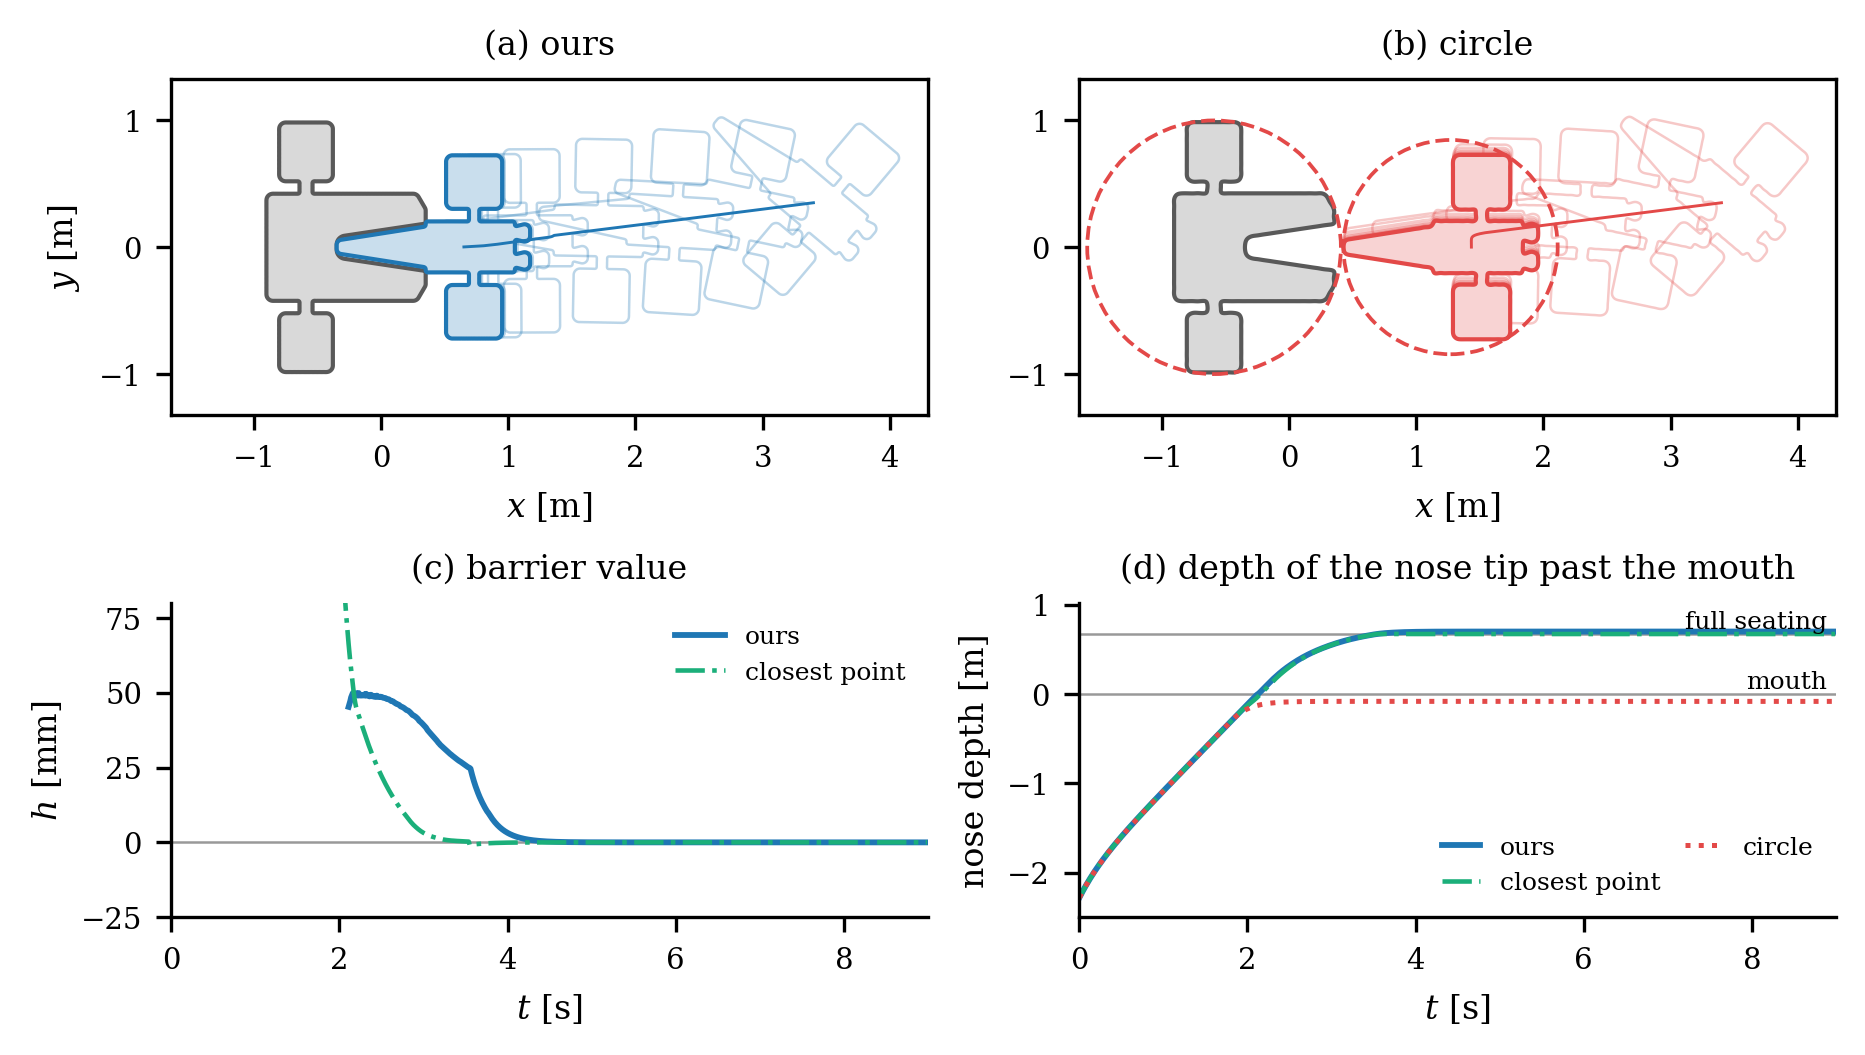
\includegraphics[width=\textwidth]{dock_paper.png}
\caption{Docking into a tapered receptacle with the module fixed. (a) Surface-cover barriers: the
vehicle rotates while approaching and seats its 0.70-m nose 3.0~cm past full seating, 1.7~mm from the
receptacle floor. (b) Minimum enclosing circles (dashed): the vehicle stops 8~cm in front of the
mouth. Poses every 0.6~s; gray: ground truth; colored and black: certified boundaries. (c) Barrier
value (for the cover, the certified lower bound of $\tilde h$ over the active boxes): both
constructions keep $h\ge0$, the
closest-point barrier violates its constraint by 0.9~mm. (d) Depth of the nose tip past the mouth
(full seating: 0.668~m).}
\label{fig:dock}
\end{figure*}

\begin{table}[t]
\caption{Docking with Different Barriers}
\label{tab:dock-base}
\centering
\footnotesize
\setlength{\tabcolsep}{1.6pt}
\renewcommand{\arraystretch}{1.05}
\begin{tabular}{lccccc}
\toprule
& \multicolumn{3}{c}{ours} & closest & \\
\cmidrule(lr){2-4}
& surface & compiled & compiled & point & circle\\
& cover & (B-spline) & ($C^0$ B\'ezier) & & \\
\midrule
certified level [mm] & 1.2, 0.5 & 12.3 & 19.0 & -- & --\\
nose depth [m] & 0.698 & 0.666 & 0.692 & 0.671 & $-0.084$\\
min.\ true gap [mm] & 1.7 & 24.8 & 6.1 & 28.4 & 102.5\\
min.\ $h$ [mm] & \textbf{0.0} & \textbf{0.0} & $-15.8$ & $-0.9$ & --\\
input variation & 6.4 & 3.6 & 161 & 3.8 & 2.5\\
constraints, max. & 1604 & 1 & 1 & 1 & 1\\
time per step [ms] & 6.2 & 0.48 & 0.49 & 6.5 & 0.22\\
\bottomrule
\end{tabular}
\\[3pt]
\parbox{\columnwidth}{\footnotesize Nose depth: tip past the mouth at the end (full seating with a
32-mm gap: 0.668~m). Cover: levels of the module and vehicle fields, 1548 boxes of 5~mm, at most 401
active; $h$: certified lower bound of $\tilde h$. Compiled
fields: $82^2{\times}384$ and $30^3$ cells. Time: median, complete filter, one CPU thread. The circle
barrier's $h$ is in m$^2$ and stayed nonnegative.}
\end{table}

With the surface cover, the vehicle docks without violating its barrier and without slack
(Fig.~\ref{fig:dock}a, Table~\ref{tab:dock-base}): it rotates while approaching, and its nose passes
the full-seating depth by 3.0~cm, closing the 32-mm floor gap to 1.7~mm. This equals the sum of the
two certified levels (1.2 and 0.5~mm), because the planar fields are fitted to exact polygon distances,
so each certified curve lies about its level away from its polygon; the 5-mm boxes cost no visible clearance, as
Proposition~\ref{prop:tight} predicts, and halving them to 2.5~mm changes the gap by 0.1~mm. Barriers at the box corners that bound $\phi_B$ alone, whose safe set
depends on the boxes, stop the nose at 6.8~mm (3.9~mm with 2.5-mm boxes). The price is up to 401 active boxes with 1604 constraints.

The compiled field docks as smoothly with a single barrier and an order of magnitude less time per step,
but its level absorbs the error of the rasterized training targets (Sec.~\ref{sec:exp-repr}): the nose
stops 2~mm short of full seating at $h=0$, with a ground-truth gap of 24.8~mm. Both $C^0$
fields push the nose deeper only by violating their constraints by 15.8 and 9.6~mm, with the
constraint normal switching across cell faces and the input chattering (total variation 161 and
94.5, against 3.6). The closest-point barrier docks as smoothly here, because the contact stays on
the tapered walls and the closest pair does not jump, but costs 13 times more per step than the
compiled field; the circles stop the nose 8~cm in front of the mouth. Refining the step from 10 to 1~ms leaves the compiled barrier
nonnegative and the final pose unchanged, whereas the violation of the $C^0$ field stays at
15--16~mm: it is caused by gradient jumps, not by discretization.

\subsection{Multiple Robots}\label{sec:exp-five}
Five shapes are generated as star-shaped radial Fourier series with hull-area ratios below 0.9,
and scaled to radii of 0.85--1.08~m. The surface cover needs one field per body: the five
tightest levels (0.29--0.35~mm) and covers (1240--1426 boxes), with the Taylor data of the boxes, take
50~s in total, an offline cost
linear in the number of bodies. The compiled construction needs one field per pair: after certified
B-spline boundaries (offsets 8--20~mm), the ten pair fields with about 6-cm cells are certified in
11--16~s each at levels of 17--26~mm, including band and regularity. The robots move to the
antipodal positions on a circle of radius 4~m under $SE(2)$ single-integrator dynamics, with start
and goal angles perturbed by up to $9^\circ$ and $20^\circ$ to avoid the central deadlock of exactly
antipodal goals. With the surface cover, all robots reach their goals after 12.5~s
(Fig.~\ref{fig:five}); the minimum ground-truth distance is 0.8~mm, and the certified lower bound of
the lifted barriers stays above $+0.17$~mm. While all five crowd the center, up to 2716 constraints
are active, and the cost per step rises from 2.8~ms (median) to 22~ms (95th
percentile). With the compiled fields, the robots arrive
after 11.9~s at 1.2/2.5~ms per step, keep 20.0~mm, and the minimum active $h$ is $-1.1$~mm, a
discrete-time effect.

\begin{figure}[t]
\centering
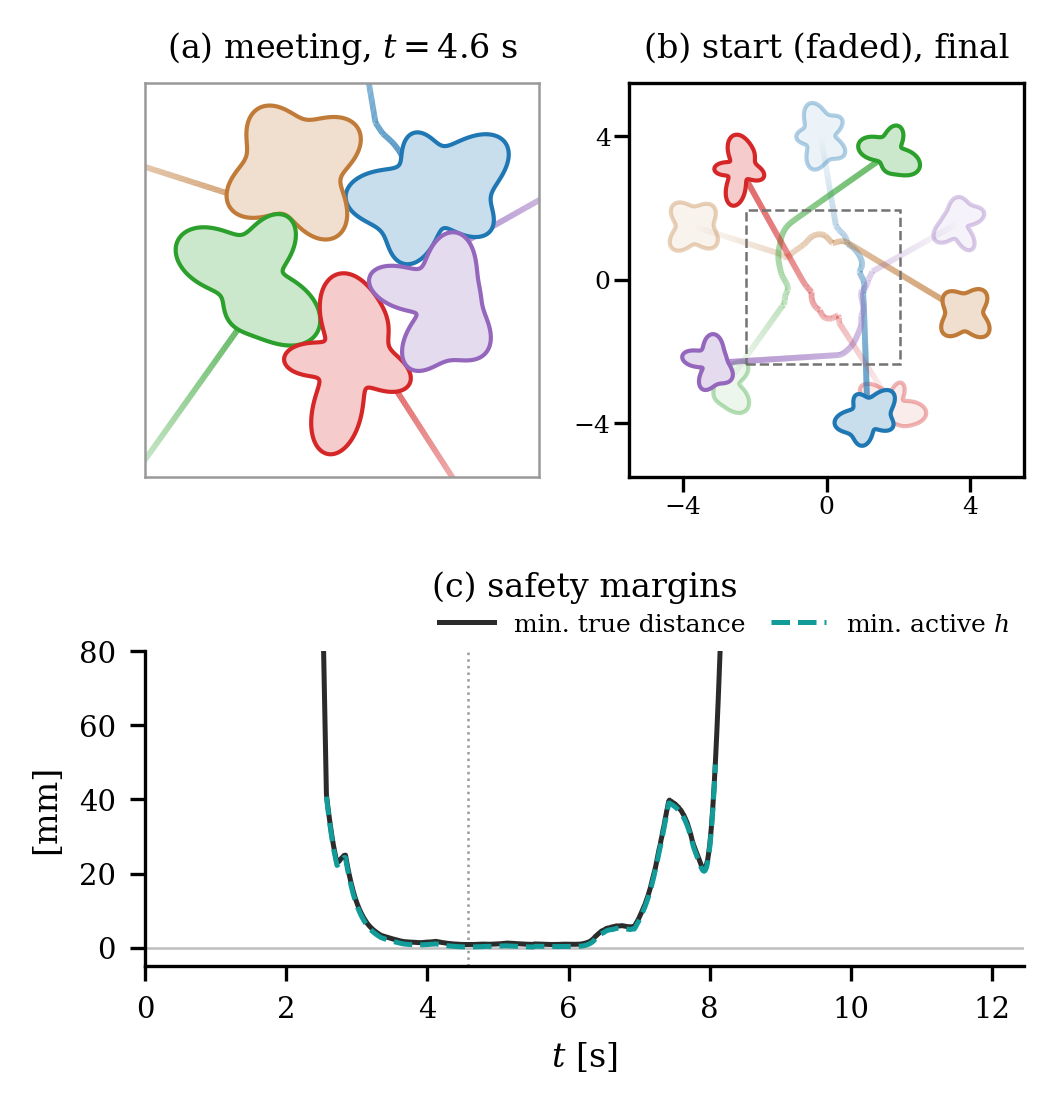
\includegraphics[width=0.92\columnwidth]{five_paper.png}
\caption{Five robots with random non-convex shapes exchanging positions under the surface-cover
barriers (gray: ground truth; colored: certified level curves). (a) Start (faded) and final poses
with center paths, drawn from faint (start) to strong (end). (b) Minimum ground-truth distance over
all pairs and certified lower bound of the lifted barriers $\tilde h$ over the active boxes.}
\label{fig:five}
\end{figure}

\begin{table}[t]
\caption{Twenty Random Five-Robot Instances}
\label{tab:stats}
\centering
\footnotesize
\setlength{\tabcolsep}{2pt}
\renewcommand{\arraystretch}{1.05}
\begin{tabular}{lcccc}
\toprule
& \multicolumn{2}{c}{ours} & closest & \\
\cmidrule(lr){2-3}
& cover & compiled & point & circle\\
\midrule
instances with a collision & \textbf{0} & \textbf{0} & 5 & \textbf{0}\\
min.\ true distance [mm] & $+0.6$ & $+19.7$ & $-86.8$ & $+42.7$\\
min.\ $h$ [mm] & \textbf{0.0} & $-2.4$ & $-114.4$ & --\\
instances, all goals reached & 12 & 13 & 12 & \textbf{20}\\
constraints, max. & 1020 & 10 & 10 & 10\\
time/step, med./max.\ [ms] & 2.0/10.2 & 0.59/7.4 & 2.5/18.7 & 0.38/0.8\\
\bottomrule
\end{tabular}
\\[3pt]
\parbox{\columnwidth}{\footnotesize Horizon 15~s, step 10~ms. Negative distances: depth of the
deepest vertex inside the other polygon. Cover: $h$ is the certified lower bound of $\tilde h$ over the
active boxes. No step required slack. Time: median over instances of the
per-instance median, and maximum; one CPU thread.}
\end{table}

With the same shapes at half size, 20 random instances with poses in $[-3,3]^2\times\Sone$ compare
the barriers under single-integrator dynamics (Table~\ref{tab:stats}). The closest-point barrier
collides in 5 instances, with vertices up to 87~mm inside the other body: the closest pair of
non-convex bodies jumps, the derivative is one-sided, and the constraint normal can point the wrong
way just before contact. These results concern this single-closest-pair construction, the one
analyzed in~\cite{jo2026geometry}, not nonsmooth formulations over all active features. Both of our
constructions and the circles never collide; the circles reach all goals, whereas the surface cover
and the compiled fields deadlock in 8 and 7 instances, mostly the same ones, because exact
non-convex boundaries can hook where round surrogates slide past. On the 11 instances completed by all
methods, path lengths differ by less than 1\% and times by less than 10\%, the surface cover being the
slowest because its remainders restrict the speed of bodies that slide close to each other: the
benefit of exact geometry appears in tight interactions such as docking. The surface cover lets the
robots pass within 0.6~mm, thirty times closer than the compiled fields, and the certified lower
bounds of its lifted barriers stay nonnegative; it uses up to 255 active boxes (1020 constraints),
and its cost per step is about three times that of the compiled fields, with a maximum of 10.2~ms.
The offline cost for these half-size bodies is 14.5~s in total, against 11--16~s for each of the
ten pairs of compiled fields. In 8 instances the compiled barrier dips below zero, by at
most 2.4~mm, when several pairs are active at full speed, while the ground-truth distance stays
above 19.7~mm owing to the certified levels. In unicycle swaps of two and four robots with the
compiled fields, no instance
collides (minimum distances 10.6 and 20.1~mm), the barrier's input coefficient norm stays above 0.128
whenever $h<5$~cm, and no step requires slack; head-on and diagonal swaps deadlock.

\subsection{Static Obstacles}\label{sec:exp-static}
The compiled construction encodes a union of static obstacles in one field and one barrier: with one
field for a robot among $m\in\{1,3,5,7\}$ random non-convex obstacles
($122\times122\times48$ cells, 2-cm training raster, $l^\star=39$--41~mm), all runs are
collision-free, and the online cost stays at 0.37--0.45~ms regardless of $m$, whereas the
closest-point baseline needs one distance computation per nearby obstacle and grows to 2.8~ms
(median) with seven.

A rocket-shaped robot (0.54~m long, nose, fuselage, two fins) escapes a curved maze (Fig.~\ref{fig:static}). The passage is our own design: three horizontal passes,
each with a smooth wiggle, joined by semicircular hairpins of radius 1.1~m, with a half-width of
0.43--0.51~m, entering and leaving the $8.9\times8.9$-m frame at right angles. The two wall regions
are the frame minus this passage, combined through a smooth maximum of signed distances so that all
corners are rounded; their ground truth consists of cubic spans, sampled into polygons with a
certified chord deviation below 0.1~mm. For the surface cover, one bivariate field with 1.25-cm cells
($791\times791$) encodes both walls, with a tightest level of 0.61~mm certified on the cubic spans
(Proposition~\ref{prop:level}, with the chord bound added to the piece radius), and the rocket's
field (1-cm cells, level 1.43~mm) is covered by 383 boxes of 5~mm. The nominal controller moves
toward eight waypoints whose straight connections cut into the walls by up to 10~cm, so the barriers
keep the rocket off the walls: they modify the nominal input in 41\% of the 3251 steps while the
rocket slides along the walls to the exit in 32.5~s (path length 23.5~m), with up to 126 active boxes
(504 constraints). The ground-truth distance at the steps is at least 4.5~mm, and a conservative audit
that subtracts half of each step's motion verifies at least 0.5~mm between steps; the certified lower
bound of $\tilde h$ on the active boxes stays above 2.4~mm, and the online cost is
2.2~ms per step (median; 95th percentile 3.6~ms).
A compiled field over the same maze ($160\times160\times48$ cells; rocket and walls enclosed by
B-splines with 64, 5825, and 5844 control points; $l^\star=44.3$~mm certified in 45~s) also escapes, in 33.0~s, but keeps
at least 17.3~mm from the walls and dips to $-0.3$~mm.

\begin{figure}[t]
\centering
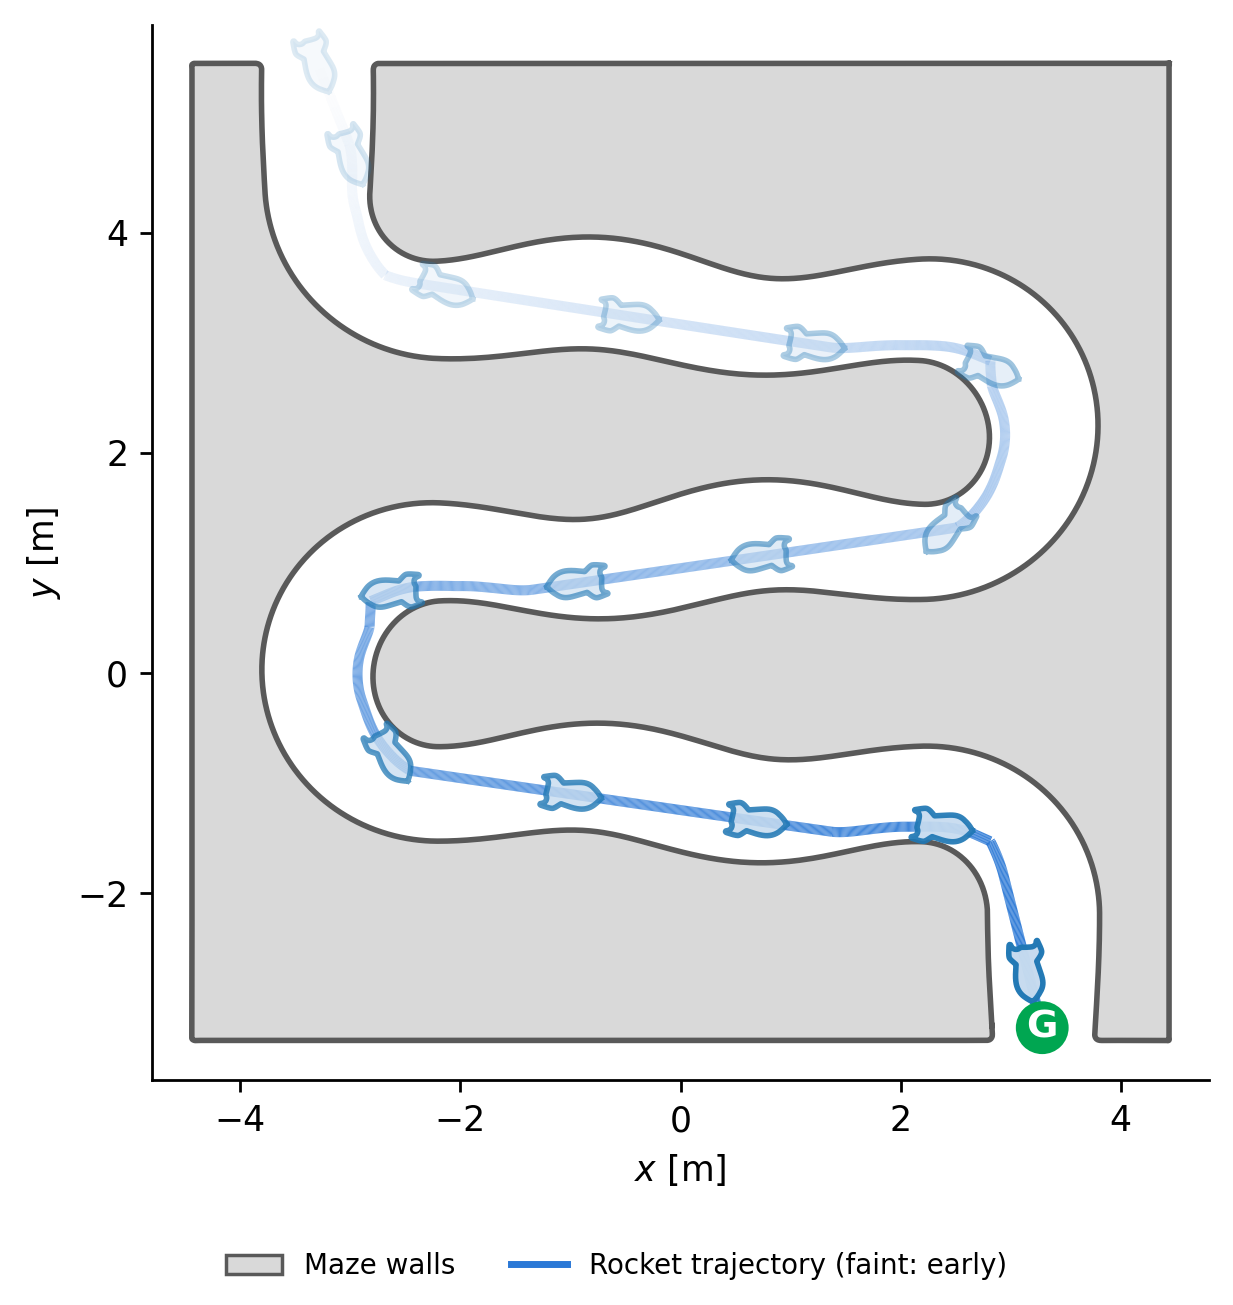
\includegraphics[width=0.8\columnwidth]{rocket_maze.png}
\caption{Escape of a rocket-shaped robot through a curved maze with surface-cover barriers and eight
goal waypoints, from the top entrance to the exit G. Gray with red outlines: walls (ground truth and
certified level curve); gray with blue outlines: the rocket at intermediate times (ground truth and
certified level curve); blue: path of its reference point. Poses and path are drawn from faint
(start) to strong (end).}
\label{fig:static}
\end{figure}

\emph{Sampling-based and ball-world baselines.} On a fixed-orientation benchmark (a cross-shaped robot
passing a cross-shaped obstacle, six approaches), adaptations of the sampling-based
barrier~\cite{lutkus2025sampling} and the ball-world controller~\cite{notomista2021nonconvex} do not
collide either; the former matches the 29.4-mm gap of our compiled field (0.106~ms per step) only with
1024 samples (0.207~ms), and the latter needs 0.217~ms with a ten times larger input variation.

\subsection{Franka Panda among Non-Convex Obstacles}\label{sec:exp-franka}
The surface-cover barriers of Sec.~\ref{sec:cover} are applied to a 7-DOF Franka Panda with the link
meshes and kinematics of~\cite{li2024representing}. All eight links (the hand, without fingers, and
links 1--7) are constrained against three non-convex obstacles made of rounded boxes: a gate, an
inverted J, and a plate carrying a 2.4-cm rod on a leg, i.e., 24
link--obstacle pairs. Each link SDF is a cubic B-spline with 12-mm cells, fitted to approximate
signed distances of its mesh; its tightest level (1.8--3.8~mm) is certified on the mesh by
Proposition~\ref{prop:level} in 0.3--2~s, and its certified surface is covered by 1440--4420 boxes of
side 6~mm ($r=5.2$~mm). The obstacle fields have 2-cm cells, tightest levels of 1.9--2.9~mm, and
domains extending 15~cm beyond the obstacles. The joints are velocity-controlled ($|\dot q_j|\le1$~rad/s) with a proportional
joint-space nominal controller, $\gamma=5$, a 10-ms step, and activation threshold $\eta=3$~cm.

Start and goal configurations are drawn uniformly within 80\% of the joint ranges with the hand
above 0.1~m and a clearance of at least 3~cm, and we keep the first 30 pairs whose unfiltered motion
collides. Safety is evaluated without sampling: the link meshes are subdivided to edges below 4~mm
(same surface), and the exact obstacle SDF at each triangle centroid minus the triangle radius
lower-bounds the distance between every mesh and every obstacle. As baselines, we use the 54
collision spheres of the Franka model in~\cite{li2024representing} and about 256 surface samples per
link, as in the collision-avoidance experiments of~\cite{li2024representing}, each with one barrier
per primitive and obstacle, the \emph{exact} obstacle SDF, and a 1-cm margin.

\begin{figure*}[t]
\centering
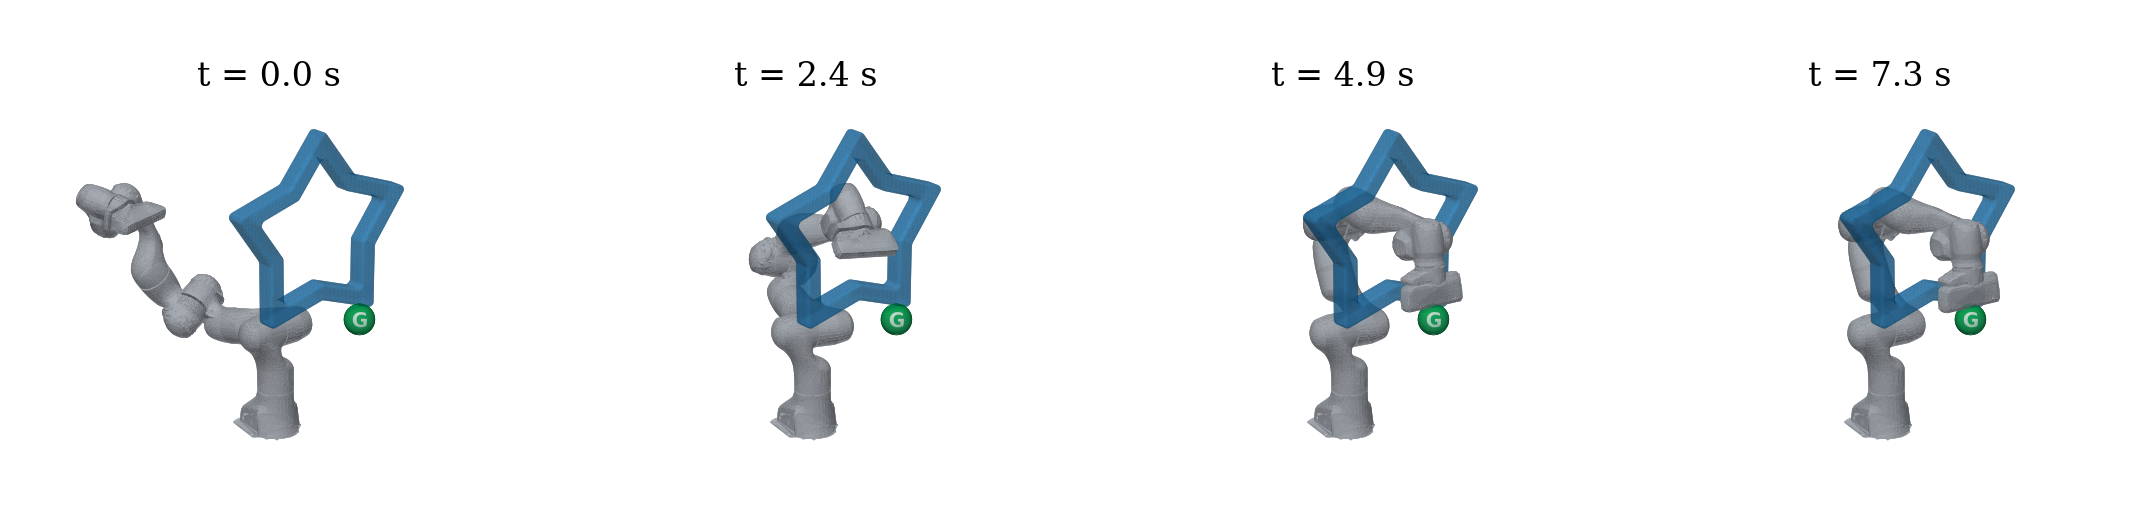
\includegraphics[width=\textwidth]{star_paper.png}
\caption{Franka Panda threading its forearm through a star-shaped tube (blue; 5-pointed star hole,
walls of constant 5-cm thickness, 6.7~cm deep) with the surface-cover barriers of all eight links.
The hand is within 1~cm of the goal G after 4.1~s; the last frame shows the settled pose. Without the
filter, the same motion cuts through the tube wall by 30.6~mm.}
\label{fig:star}
\end{figure*}

\begin{table}[t]
\caption{Franka Panda: 30 Trials Whose Unfiltered Motion Collides}
\label{tab:franka}
\centering
\footnotesize
\setlength{\tabcolsep}{2pt}
\renewcommand{\arraystretch}{1.05}
\begin{tabular}{lcccc}
\toprule
& ours & spheres & samples & KKT\\
\midrule
primitives & 26{,}636 & 54 & 1975 & 24\\
certified guarantee & yes & no & no & no\\
trials with a collision & \textbf{0} & 0 & 0 & 7\\
\quad without margin & -- & 17 & 19 & --\\
\quad deepest penetration [mm] & -- & 10.2 & 13.4 & 41.9\\
certified min.\ distance [mm] & 1.1 & 0.9 & 1.4 & $<0$\\
median of the minima [mm] & 5.7 & 8.6 & 7.2 & 2.4\\
trials reaching the goal & 17 & 20 & 23 & 20\\
trials needing slack & 0 & 0 & 0 & 7\\
time/step, med./p95 [ms] & \timeOurs & \timeSph & \timePts & \timeKKT\\
constraints, max. & 34{,}992 & 21 & 188 & 5\\
\bottomrule
\end{tabular}
\\[3pt]
\parbox{\columnwidth}{\footnotesize Without the filter, all 30 trials collide. Primitives: boxes,
spheres, surface samples, and closest-point pairs. Spheres and samples: exact obstacle SDF with a
1-cm margin unless stated; KKT: the certified fields and levels of ours. Distances: certified lower
bounds between the link meshes and the obstacles. Time per step: median and 95th percentile over all steps of the 30 trials, one CPU thread
(Python, AMD Ryzen~9 3900X).}
\end{table}

In all 30 trials, our filtered arm is collision-free (Table~\ref{tab:franka}), with a certified
minimum distance of 1.1~mm between meshes and obstacles (median over trials 5.7~mm); no step
requires slack, and the certified lower bounds of the lifted barriers stay nonnegative. Each certified
surface encloses its mesh at a distance between zero and roughly its level, depending on the local
fitting error, so the meshes can come closer than the sum of the two levels (at least 3.7~mm), and the
6-mm boxes add no visible clearance (Proposition~\ref{prop:tight}); barriers at the box corners that
bound $\phi_O$ alone kept 8.4~mm in the same trials. Within the 10-s horizon, the arm reaches the goal in 17 trials, against
23 with those corner barriers: close to an obstacle, the remainders of~\eqref{eq:coef} slow the links
that slide along it, and in the other trials the arm stops in front of an obstacle. The filter needs
\timeFrankaMed~ms per step (median; 95th percentile \timeFrankaPninetyfive~ms) with up to 4374 active
boxes (34{,}992 constraints).

With a 1-cm margin, neither baseline collides in these trials, but both come within about 1~mm of
the obstacles (0.9 and 1.4~mm): the margin, not a certificate, absorbs the geometric error of the
primitives. Without the margin, the spheres collide in 17 of the 30 trials, by up to 10.2~mm,
because they do not enclose the meshes, and the surface samples collide in 19, by up to 13.4~mm,
although every sampled barrier stays above $-0.05$~mm: the obstacle enters between the samples. The baselines are
cheaper per step and reach the goal more often (20 and 23 trials); what the surface cover adds is
that the constraint holds on the whole continuous surface, so that no margin has to be tuned.
Finally, the closest-point barrier of~\cite{jo2026geometry}, transferred to 3D with the same
certified fields and levels (one barrier per link--obstacle pair at
$\mathbf x^\ast=\argmin\phi_O$ subject to $\phi_A=l_A$, SLSQP warm-started from the previous step),
collides in 7 trials by up to 41.9~mm, violates its own barrier by up to 37~mm, needs slack in 7, and
costs 128~ms per step:
on non-convex links the closest point is only a local minimizer and jumps between surface patches,
as in the planar comparison.

\emph{Threading a star-shaped tube.} Fig.~\ref{fig:star} shows a tighter static scene, arranged in an
interactive tool and replayed: a tube whose hole is a 5-pointed star (tips at 24~cm, notches at
15~cm), surrounded by walls of constant 5-cm thickness and 6.7~cm deep, stands 0.65~m high in front of
the arm. Its ground truth is the extruded star-minus-star region, whose exact SDF is analytic; its
field has 1.5-cm cells and a tightest level of 3.9~mm. The arm starts beside the tube and a
damped-least-squares IK moves the hand to the home pose, which puts the forearm through the hole.
Without the filter, the motion cuts through the tube wall by up to 30.6~mm and stays in contact for
10.2~s. With it, the arm threads its forearm through the star hole and reaches the home pose after
4.1~s, with a certified clearance of at least 3.0~mm and no slack. Near the sharp edges of the star,
$\phi_O$ varies quickly, and refining only the boxes within 1~cm lets the arm freeze at the rim; in
this scene, every active box whose remainder exceeds $\vartheta$ is refined, with up to 5410 active
boxes (43{,}280 constraints) and 96~ms per step (median; 95th percentile 109~ms).

\subsection{Two Franka Pandas in a Shared Workspace}\label{sec:exp-dual}
\begin{figure*}[t]
\centering
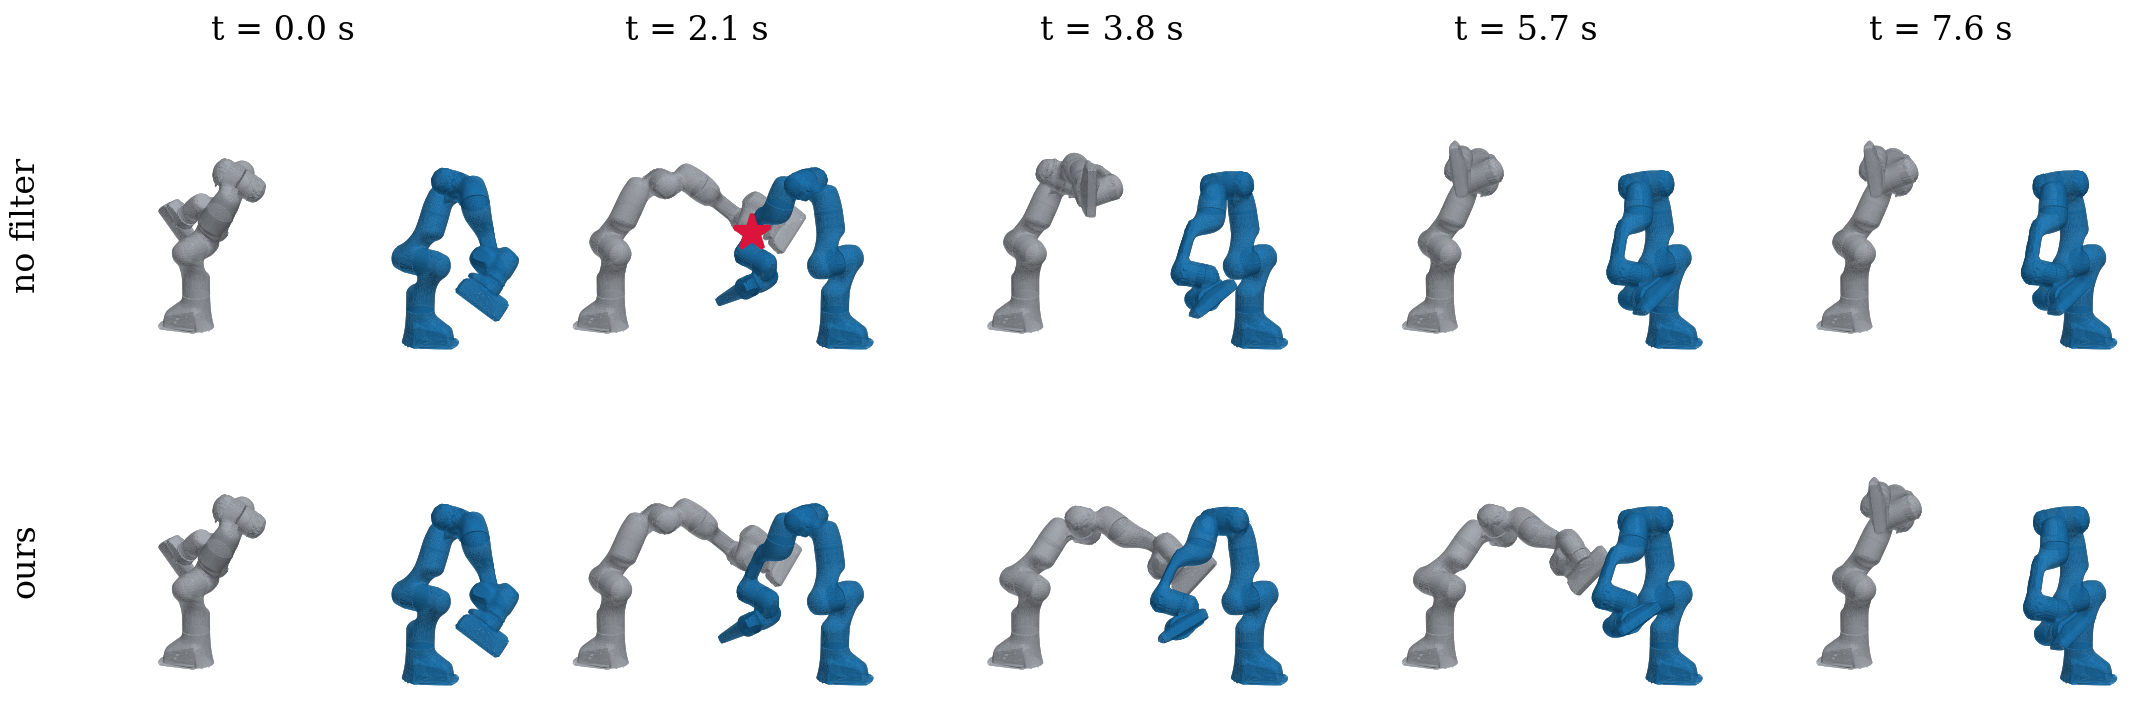
\includegraphics[width=\textwidth]{dual_paper.png}
\caption{Two Franka Pandas move to their goals and cross. Top: without the safety filter, the arms
collide (links in contact red) and pass through each other. Bottom: with the surface-cover barriers of
all 64 link pairs, arm~1 (gray) and arm~2 (blue) slide past each other and both reach their goals,
7.6~s after the start.}
\label{fig:dual}
\end{figure*}
Two Franka Pandas face each other with bases 0.9~m apart. For each of the 64 pairs of a link of arm~1
and a link of arm~2, the certified surface of the first is bounded against the SDF of the second;
both links move, so each constraint is affine in the velocities of all 14 joints (the
derivative in Sec.~\ref{sec:cover} with the Jacobians of both arms), and one direction per pair
suffices by Theorem~\ref{thm:cover}. Starts and goals of both arms are drawn as before, with an
initial clearance of 5~cm, and we keep the first 20 of 143 sampled pairs whose unfiltered motion
brings the arms into contact (sampled mesh distance below 2~mm). The distance between the arms is
bounded from below with exact point-to-triangle distances from the subdivided triangles of arm~1 to
the meshes of arm~2, at the 20 steps of each trial with the smallest sampled distance. In all 20
trials the arms stay apart without slack (Fig.~\ref{fig:dual} shows one); the barriers are active
($\min h<5$~mm) in 8 trials, the
meshes come within 3~cm of each other in 16, and the certified minimum distance is 1.6~mm, below the
sum of the two levels of a pair of links for the same reason (corner barriers on $\phi_B$ alone kept
10.3~mm). Both arms reach their
goals in 15 trials (17 with the corner barriers). The filter needs \timeDualMed~ms per step (median;
95th percentile \timeDualPninetyfive~ms) with up to 6730 active boxes (53{,}840 constraints) over the
64 link pairs.

% -----------------------------------------------------------------------------
\section{Limitations}\label{sec:limits}
\emph{Certificates.} The certificates exclude first contacts, so they protect trajectories that
start collision-free, and they certify non-intersection, not a prescribed clearance (which follows
by enclosing dilated ground truths). They assume exact arithmetic; our implementation uses double
precision without outward rounding.

\emph{Discrete time.} The guarantees hold in continuous time. With 10-ms steps, the compiled barrier
dipped to $-2.4$~mm in random swaps, whereas the certified lower bounds of the surface cover stayed
nonnegative; a sampled-data tightening is needed for the implemented controller.

\emph{Conservatism, feasibility, and cost.} The safe set of the surface cover is exact up to the two
certified levels, but its enforcement is not: the Taylor remainders and the Bernstein coefficients
restrict the admissible inputs, so the constraints can hold bodies back from the boundary of the safe
set by an amount of second order in the box size, may slow them where the fields vary quickly, and are
guaranteed feasible only outside that band. Where the third derivatives of the fields are large, as
near sharp edges, finer boxes would recover speed at the price of more constraints. Their number,
$2^n$ per active box and thousands in tight spatial scenes, sets the cost per step and its
variation. The compiled field keeps one barrier and a bounded cost per pair, but its level is
limited by the training targets; spatially varying levels would reduce it.

\emph{Scope.} Deadlocks are not resolved, and exact geometry makes them more frequent than round
surrogates. The compiled construction is limited to low-dimensional relative poses and needs one
field per pair of shape types. The manipulator studies omit self-collision within an arm, the
fingers, and polytopic baselines, and all experiments are in simulation.

% -----------------------------------------------------------------------------
\section{Conclusion}\label{sec:concl}
Collision avoidance between non-convex rigid bodies reduces, through a first-contact lemma, to
keeping each body's SDF above a certified level on the boundary of the other. We took this condition
on the continuous level set as the safe set and enforced it through Bernstein bounds of a lifted
barrier on a cover of that level set, so that the finite certificate restricts only the inputs, for
planar and spatial, rigid and articulated bodies; for planar pairs, we also compiled it into one
configuration-space field per pair, certified by a Bernstein branch-and-bound. Neither construction
computes closest points, and both certify enclosure of the true geometry. Both never collided in
planar experiments, unlike a closest-point barrier, and docked where bounding circles cannot; the
surface cover kept a Franka Panda off three non-convex obstacles and two Pandas apart, within the
certified levels. Sampled-data guarantees, faster enforcement near contact, deadlock resolution, and
hardware validation are the next steps.

\bibliographystyle{IEEEtran}
\bibliography{references}

\end{document}
